% Options for packages loaded elsewhere
\PassOptionsToPackage{unicode}{hyperref}
\PassOptionsToPackage{hyphens}{url}
%
\documentclass[
  11pt,
  a4paper,
]{article}
\usepackage{amsmath,amssymb}
\usepackage{lmodern}
\usepackage{iftex}
\ifPDFTeX
  \usepackage[T1]{fontenc}
  \usepackage[utf8]{inputenc}
  \usepackage{textcomp} % provide euro and other symbols
\else % if luatex or xetex
  \ifXeTeX
    \usepackage{zxjatype} 
    \usepackage[ipaex]{zxjafont}
    \setromanfont{Times New Roman}
  \fi
  \usepackage{unicode-math}
  \defaultfontfeatures{Scale=MatchLowercase}
  \defaultfontfeatures[\rmfamily]{Ligatures=TeX,Scale=1}
\fi
% Use upquote if available, for straight quotes in verbatim environments
\IfFileExists{upquote.sty}{\usepackage{upquote}}{}
\IfFileExists{microtype.sty}{% use microtype if available
  \usepackage[]{microtype}
  \UseMicrotypeSet[protrusion]{basicmath} % disable protrusion for tt fonts
}{}
\usepackage{xcolor}
\IfFileExists{xurl.sty}{\usepackage{xurl}}{} % add URL line breaks if available
\IfFileExists{bookmark.sty}{\usepackage{bookmark}}{\usepackage{hyperref}}
\hypersetup{
  hidelinks,
  pdfcreator={LaTeX via pandoc}}
\urlstyle{same} % disable monospaced font for URLs
\usepackage[left=3cm,right=3cm,top=3cm,bottom=3cm]{geometry}

\usepackage{setspace}
\renewcommand{\baselinestretch}{1.5}
\usepackage{float}

\usepackage{longtable,booktabs,array}
\usepackage{threeparttable, threeparttablex, multirow}
\usepackage{calc} % for calculating minipage widths
% Correct order of tables after \paragraph or \subparagraph
\usepackage{etoolbox}
\makeatletter
\patchcmd\longtable{\par}{\if@noskipsec\mbox{}\fi\par}{}{}
\makeatother
% Allow footnotes in longtable head/foot
\IfFileExists{footnotehyper.sty}{\usepackage{footnotehyper}}{\usepackage{footnote}}
\makesavenoteenv{longtable}
\renewcommand{\figurename}{図}
\renewcommand{\tablename}{表}
\usepackage{graphicx}
\makeatletter
\def\maxwidth{\ifdim\Gin@nat@width>\linewidth\linewidth\else\Gin@nat@width\fi}
\def\maxheight{\ifdim\Gin@nat@height>\textheight\textheight\else\Gin@nat@height\fi}
\makeatother
% Scale images if necessary, so that they will not overflow the page
% margins by default, and it is still possible to overwrite the defaults
% using explicit options in \includegraphics[width, height, ...]{}
\setkeys{Gin}{width=\maxwidth,height=\maxheight,keepaspectratio}
% Set default figure placement to htbp
\makeatletter
\def\fps@figure{htbp}
\makeatother
\setlength{\emergencystretch}{3em} % prevent overfull lines
\providecommand{\tightlist}{%
  \setlength{\itemsep}{0pt}\setlength{\parskip}{0pt}}
\setcounter{secnumdepth}{5}
\newlength{\cslhangindent}
\setlength{\cslhangindent}{1.5em}
\newlength{\csllabelwidth}
\setlength{\csllabelwidth}{3em}
\newlength{\cslentryspacingunit} % times entry-spacing
\setlength{\cslentryspacingunit}{\parskip}
\newenvironment{CSLReferences}[2] % #1 hanging-ident, #2 entry spacing
 {% don't indent paragraphs
  \setlength{\parindent}{0pt}
  % turn on hanging indent if param 1 is 1
  \ifodd #1
  \let\oldpar\par
  \def\par{\hangindent=\cslhangindent\oldpar}
  \fi
  % set entry spacing
  \setlength{\parskip}{#2\cslentryspacingunit}
 }%
 {}
\usepackage{calc}
\newcommand{\CSLBlock}[1]{#1\hfill\break}
\newcommand{\CSLLeftMargin}[1]{\parbox[t]{\csllabelwidth}{#1}}
\newcommand{\CSLRightInline}[1]{\parbox[t]{\linewidth - \csllabelwidth}{#1}\break}
\newcommand{\CSLIndent}[1]{\hspace{\cslhangindent}#1}


\usepackage{float}
\usepackage{booktabs}
\usepackage{longtable}
\usepackage{array}
\usepackage{multirow}
\usepackage{wrapfig}
\usepackage{colortbl}
\usepackage{pdflscape}
\usepackage{tabu}
\usepackage{threeparttable}
\usepackage{threeparttablex}
\usepackage[normalem]{ulem}
\usepackage{makecell}
\usepackage{xcolor}
\ifLuaTeX
  \usepackage{selnolig}  % disable illegal ligatures
\fi

\makeatletter
\def\@fnsymbol#1{\ensuremath{\ifcase#1\or \dagger\or \ddagger\or
   \mathsection\or \mathparagraph\or \|\or **\or \dagger\dagger
   \or \ddagger\ddagger \else\@ctrerr\fi}}
    \makeatother

\date{}



\begin{document}

\newpage
\thispagestyle{empty}
\phantom{a}
\newpage

\hypertarget{intro}{%
\section{はじめに}\label{intro}}

季節性インフルエンザ・新型コロナウイルス・風しんなどの感染症は、
感染した本人の健康状態を悪化させるだけでなく、感染者本人から他者に感染させてしまう特性をもっている。
ワクチンはこのような感染症の有効な対策の一つである。
ワクチンは感染予防効果(感染そのものを防ぐ)と発症予防効果(感染しても発症を防ぐ)を持っている\footnote{ワクチンは感染予防効果・発症予防効果に加えて、重症感染予防効果(感染して発症しても重症化を防ぐ)を持っているものがある。}。
季節性インフルエンザやCOVID-19に対するワクチンは主に発症予防効果を持っている一方で、
本研究が焦点を当てる風しんに対するワクチンは主に感染予防効果を持っている。
感染予防効果を持つワクチン接種は正の外部性を持っている。
ワクチン接種に正の外部性があれば、
人々が利己的に意思決定をしているとワクチン接種は社会的に最適な水準より過小となってしまう。
なぜなら、個人の限界便益は外部性の限界便益を含めた社会的限界便益を下回るからである。
また、自分の接種が他者の感染確率を引き下げるという社会的便益を考慮して意思決定をしていたとしても、
他者がワクチンを接種してくれると自分の感染確率が下がるだけではなくまた別の人への感染確率も下がるため
フリーライダーの問題が発生する(Ibuka et al., 2014)。

こうした特徴は、社会的に最適な接種水準を達成するために政府の介入を正当化する。
伝統的な経済学はワクチン接種に対する補助金(ピグー補助金)を政府介入の一つとして挙げている。
たとえば、多くの国で、COVID-19に対するワクチン接種は無料で受けられる。
また、日本では、予防接種法で規定されている定期接種は原則として自己負担がない。
これはワクチン接種の補助金政策とみなすことができる。
さらに、ワクチン接種補助金は、ワクチンを接種した人に対して金銭やくじ券を配布する政策のように
接種無料化に必要な金額を超えて設定されることある。
たとえば、アメリカのニューヨーク市では、
1回目のCOVID-19のワクチンを接種した人に対して100ドルの金銭を与えている。
いくつかの研究では、金銭やくじ券を配布する政策がワクチン接種を促進することを示している\footnote{Barber and West (2022) や Brehm et al. (2021) によると、アメリカのオハイオ州がCOVID-19のワクチンを接種した人に560万ドルがあたるくじ券を配布し、
  それがワクチン接種を促進したことを明らかにしている。
  また、Campos-Mercade et al. (2021) は金銭的インセンティブの効果をランダム化比較試験(RCT)で検証し、ワクチン接種率を4\%ポイント高めたことを報告している。
  COVID-19のワクチン接種以外にも、金銭的インセンティブがインフルエンザワクチン(Bronchetti et al., 2015)や
  発展途上国における子供の免疫獲得(Banerjee et al., 2010; Barham and Maluccio, 2009)を促進することを明らかにしている。}。

このような従来の政策に加えて、
行動経済学の知見に基づくナッジの活用が、ワクチン接種を促進するための政策として近年注目されている。
セイラーとサンスティーン (2009) はナッジを
「選択を禁じることも、経済的なインセンティブを大きく変えることもなく、人々の行動を予測可能な形で変える選択アーキテクチャーのあらゆる要素」
と定義している。
ワクチン接種における代表的なナッジとして、
選択肢の提示の仕方を変える政策やリマインダーを送付する政策が挙げられる\footnote{Chapman et al. (2010) は「どの日付で接種の予約するか」というオプト・インの選択肢よりも
  「指定された接種予約をキャンセルするかどうか」というオプト・アウト選択肢を提示する方が、
  インフルエンザのワクチン接種を促進できることを明らかにした。
  また、Milkman et al. (2021) や Dai et al. (2021) は
  インフルエンザやCOVID-19のワクチン接種を勧奨するリマインダーがワクチン接種率を高めることを明らかにした。}。
リマインダーを送付するときに、
どのような内容でワクチン接種を勧奨するべきかという点もナッジの一つである(以降では、ナッジ・メッセージと呼ぶ)\footnote{ナッジ・メッセージはワクチン接種だけでなく、
  滞納した税金の督促状(Hallsworth et al., 2017)や滞納したクレジットカードの負債の督促状(Bursztyn et al., 2019)でも研究されている。}。
たとえば、リマインダーの内容を「あなたのためにワクチンを確保しています」という所有権を強調することで、
リマインダーの効果がより強くなることを示している(Dai et al., 2021; Milkman et al., 2021)。
所有権を強調する以外にも、いくつかの研究は、ワクチン接種による他者の便益を強調するメッセージや
自身の行動が他者の意思決定に影響を与えるという社会的影響効果を強調するメッセージも
ワクチン接種やその意向を高めることを示している\footnote{Dai et al. (2021) はワクチン接種による他者の便益を強調するようなメッセージを加えたリマインダーが
  ワクチン接種を促進したことを明らかにしている。
  ただし、これはリマインダーを送付していない群を比較対象にしているので、リマインダーの効果をより強めているかどうかは分からない。
  また、Sasaki et al. (2022) は、「あなたのワクチン接種が周囲の人のワクチン接種を後押しします」という社会的影響効果を
  強調するメッセージがワクチン接種の意向を高めることを示している。}。

ナッジを実際の政策に活用するときに、重要な論点が二つある。
第一に、ナッジの有効性に関するエビデンスが混在しているということである。
金銭的インセンティブがワクチン接種を促進することを示した
Bronchetti et al. (2015) や Campos-Mercade et al. (2021) はナッジの効果も検証し、
ナッジにはワクチン接種を促進する効果は見られなかったと報告している。
また、 DellaVigna and Linos (2020) は学術研究で示されたナッジの効果は実際の政策で用いられているナッジの効果よりも大きいことを報告している。
したがって、どのようなナッジが行動を促進するのか、
そして、学術研究で観察される効果の外的妥当性がどれだけ担保されているかは慎重に議論する必要がある。

第二に、ナッジの費用対効果や社会厚生に与える影響に関するエビデンスが不足しているという点である。
仮にあるナッジが行動を促進することを明らかにしても、
そのナッジの費用対効果が低い場合や社会厚生で評価したときに負の影響を与える場合には、
政府はそれを実際の政策に用いるべきでない。
Chetty et al. (2009) は商品の値札を税抜き価格表示と税込み価格表示を比較し、
税抜き価格表示では税金を考慮しないで消費決定することを実証的に明らかにし、
税抜き表示が消費者の厚生を下げることを示した。
その意味で、税込み価格表示というナッジが社会厚生を改善することを明らかにした。
Benartzi et al. (2017) は過去の研究結果を用いて金銭的インセンティブとナッジの費用対効果を計算し、
ナッジ政策の方が金銭的インセンティブより費用対効果が高いことを示した。
また、ナッジ政策と同等の効果を得るために必要な金銭的インセンティブの規模も費用対効果の議論に重要な指標となる。
Bursztyn et al. (2019) や Moriwaki et al. (2020) はナッジ・メッセージの効果検証と同時に、ナッジ・メッセージの金銭的価値を推定している。

本研究では、風しんワクチンの接種を促進できるナッジ・メッセージを開発するとともに、
費用対効果を含めて効果検証を行うことで、
これまでのナッジの学術的・政策的議論に新しい知見を追加することを目的とする。
風しんは感染した本人の健康状態を悪化させるだけでなく、
妊娠初期の女性に感染させてしまうと、生まれてくる幼児の目や耳、心臓に障害が起きる可能性がある。
日本では、1977年から風しんのワクチン接種は定期接種として公費負担で市町村が実施してきたが、
58歳以上の男女と40歳から57歳の男性は風しんワクチンが定期接種になっておらず、自己負担の任意接種であった\footnote{以降で示す年齢は2019年4月時点の年齢である。}。
しかし、40歳から57歳の男性は、ワクチンが任意接種であった上に自然感染による風しん感染が少なかったので、
他の世代よりも風しんの抗体保有率が低い\footnote{58歳以上の男女は、自然感染による風しんの抗体保有率が高いためワクチン接種の必要性は低い。}。
この世代の男性の風しん抗体保有率が90\%以上になれば、日本は風しんの集団免疫を獲得できる(Nishiura et al., 2015)。

そこで、風しんの集団免疫を得るために、
厚生労働省は2019年4月から2020年3月にかけて、この年齢層の男性に対して、
風しんの抗体検査とワクチン接種を無料で受けられるクーポン券を発行し、
この世代の男性の風しんの抗体保有率を抗体非保有者に対するワクチン接種を促進することで、90\%以上に高めようとした。
クーポン券は年齢別に段階的に発行され、2019年度では、40歳から46歳の男性が自動的に送付された。
一方で、47歳から57歳の男性は2020年度以降にクーポン券が送付されるが、
本人の希望もしくは市区町村の判断によって2019年度にクーポン券を受け取ることができた。
しかしながら、2019年1月時点でクーポン券を利用した抗体検査の受検率は約18\%と低かった。

このような背景を踏まえて、
本研究は、オンライン調査上でランダム化比較試験(RCT)を実施して、
風しんワクチンの接種の促進を目的にしたナッジ・メッセージの効果を評価する。
我々は日本全国に居住する厚生労働省の追加対策の対象となった世代の男性を調査対象として、
2020年2月と3月に調査を実施した。
2月の調査はコントロールを含めた7つのメッセージのうちランダムに1つを示した後、
抗体検査の受検やワクチン接種の意向を調査した。
3月の調査は第1回調査の追跡調査であり、
第1回調査の回答以降に抗体検査やワクチン接種を受けたかどうかを同一個人に対して調査した。
この二つの調査のデータを用いて、
ナッジ・メッセージの抗体検査の受検やワクチン接種の意向と行動に対する効果を推定する。

主な結果は次の通りである。
第一に、2019年度に無料のクーポン券が自治体から自動的に送付された男性において、
妊娠初期の女性に風しんを感染させることで胎児の健康が損なわれる可能性があることを
強調した利他的なメッセージは抗体検査受検の意向と行動に正の効果を持っていた。
第二に、ナッジ・メッセージの種類やクーポン券の送付の有無に関わらず、
抗体検査の結果が陰性であった(抗体を保有していない)人のほとんどが、その後ワクチンを接種していた。
このことは、抗体保有率を高めるためには、
検査後の陰性者よりも検査前の対象者に介入して検査の受検率を高めるような政策に焦点を当てるべきであり、
本研究の利他的なメッセージは風しんの抗体保有率を高めるために有効なメッセージであることを示唆している。
第三に、2019年度はクーポン券を入手するには自ら申し込む必要のあった男性において、
いずれのナッジ・メッセージも統計的に有意な効果を示さなかった。

本論文の構成は次の通りである。
第 \ref{background} 節は日本における風しん対策の背景を概観する。
第 \ref{experiment} 節はオンライン調査実験の内容を説明する。
第 \ref{result} 節で結果を示し、第 \ref{conclusion} 節で結論を述べる。

\hypertarget{background}{%
\section{日本における風しんワクチンの背景}\label{background}}

ワクチン接種には、予防接種法で規定されている定期接種とそれ以外の任意接種がある。
定期接種は原則として自己負担がないが、任意接種は接種料金を自己負担する必要がある。
1994年の予防接種法の改正により、定期接種は義務接種から努力接種へと変更された。

感染予防効果を持つ風しんワクチンは、
妊婦の感染防止のために1977年8月から定期接種の対象となった。
この時期から中学生の女子を対象に1回の定期接種が行われた。
1989年4月から、
中学生女子を対象とした定期接種と同時に、
生後12-72カ月の幼児が麻疹ワクチンの定期接種を受けるとき、
親は麻しん・おたふくかぜ・風しん混合ワクチン(MMRワクチン)を選択することができた。
しかしながら、無菌性髄膜炎の副作用の多発により、
MMRワクチンの義務接種としての定期接種は1993年4月に一旦中止された。
その後、1995年4月から経過措置とともに努力義務としての定期接種が再開された\footnote{1995年4月から、風しんの流行そのものを止めるために集団免疫の獲得を目的として、定期接種が再開され接種対象者が生後12-90カ月未満の男女に変わった。同時期に、経過措置として、以前に風しんワクチンもしくはMMRワクチンを接種していない人が接種の対象となった。経過措置の定期接種の対象者は(1)1995年度に小学校1-2年生と生後90カ月未満の男女、(2)1996-1999年度に小学校1年生、(3)1995年4月から2003年9月にかけて、1979年4月2日から1987年10月1日に生まれた中学生男女である。2006年から、麻疹風しん混合ワクチン(MRワクチン)を用いて、2回の定期接種が行われている。1回目は生後12-24カ月の幼児期であり、2回目は小学校入学前1年間の幼児期である。さらに、2007年から始まった10代・20代を中心とする麻疹の全国的な流行を受けて、2008年4月から2013年3月までにかけて、当時中学1年生および高校3年生相当の学生を対象に、MRワクチンの2回目接種の機会が設けられた。}。

その結果、日本では風しんワクチンの定期接種を受けていない2つの年齢層が生じることになった。
定期接種を受けていない世代は、(1)1962年4月2日以前に生まれた男女と
(2)1962年4月2日から1979年4月1日に生まれた男性である\footnote{(1)は1977年の風しんワクチンの定期接種が始まる前に中学校を卒業したグループである。
  (2)は風しんワクチンの定期接種の対象が中学生女子であり、1995年以降の経過措置の対象にならなかったグループである。}。
1979年4月2日以降に生まれた男女は経過措置を含めて定期接種の対象者となっているが、接種回数は年齢によって異なる。
定期接種を受けていない人は自然感染による抗体保有の可能性があるだけで、ワクチン接種による風しん抗体を保有していない。

\begin{figure}[t]
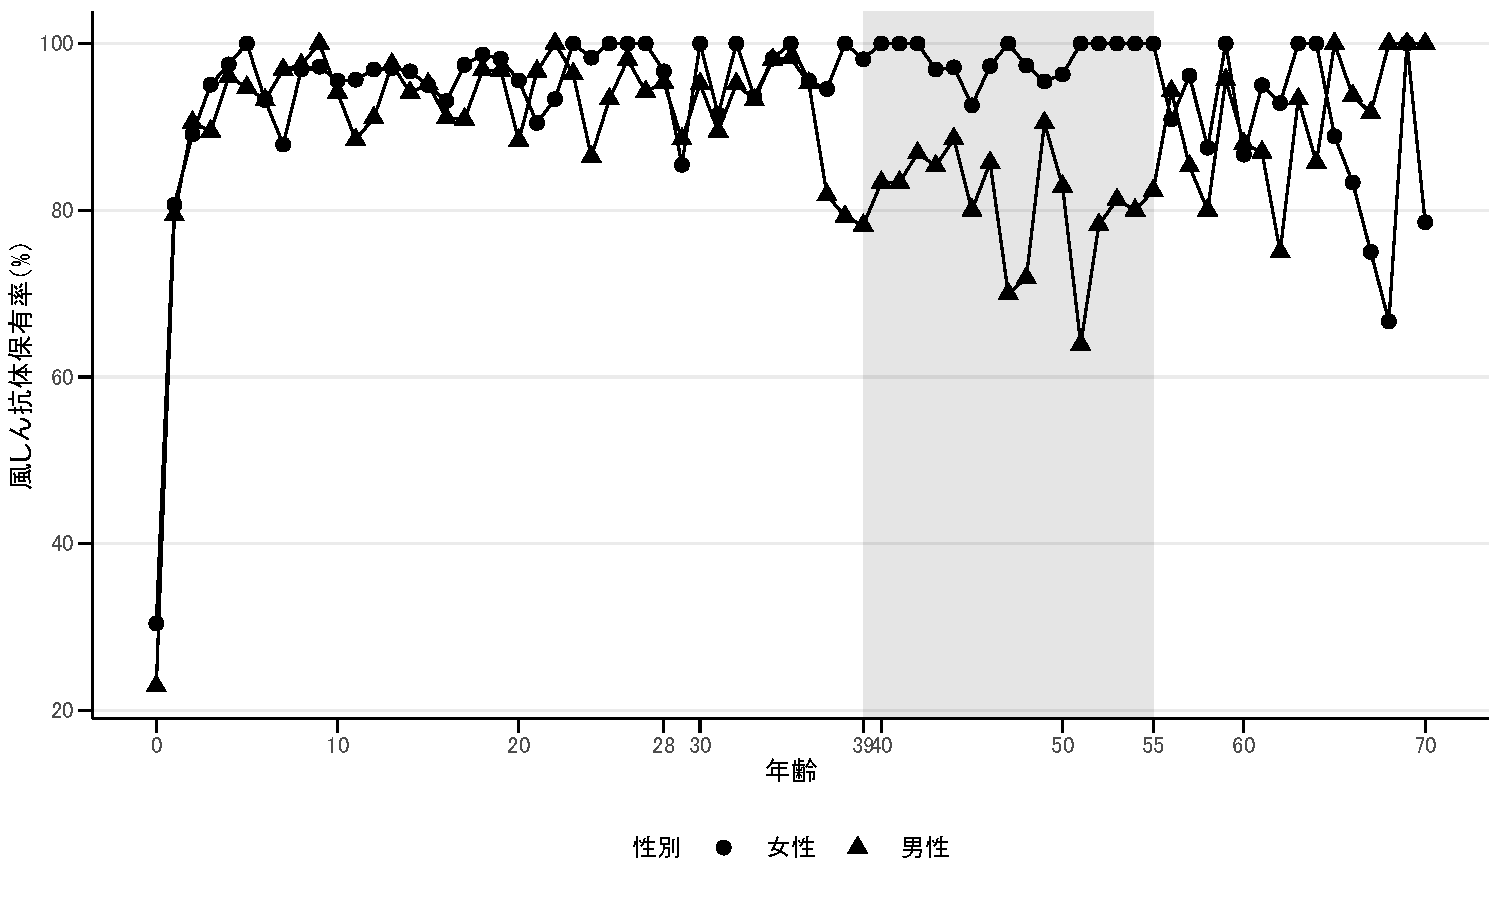
\includegraphics{C:/Users/vge00/Desktop/MHLWRubellaNudge/publish/RIETI/webRCT/webRCT_files/figure-latex/NiidAntibody-1} \caption{男女別の各年齢における風しん抗体保有率。データソース: 国立感染症研究所『2018年度感染症流行予測調査(NESVPD)』}\label{fig:NiidAntibody}
\end{figure}

風しんの抗体はワクチン接種だけでなく、自然感染でも得られる。
高齢者を中心に、風しんが流行していた期間に育った人ほど、風しんに自然感染した比率が高くなるので、
風しんワクチンを接種していなくても抗体を保有している可能性が高くなる。
図\ref{fig:NiidAntibody}は国立感染症研究所(NIID)の
2018年度感染症流行予測調査の男女別・年齢別の風しん抗体保有率をプロットしたものである。
56歳以上の各年齢の抗体保有率の平均は、男女とも約90\%である(男性:
91.3\%
、女性:
89.4\%
)。
一方、39歳以上55歳以下の(1962年4月2日から1979年4月1日生まれ)の抗体保有率の平均は、
男性では、
80.7\%
、女性では、
98.3\%
である。
つまり、この年齢層の男性の抗体保有率は同世代の女性の抗体保有率より低い。
これは39歳以上55歳以下の男性は風しんワクチンの定期接種の対象外である一方、
39歳以上55歳以下の女性は中学生のときに風しんワクチンを接種していることを反映している。
また、39歳以上55歳以下の男性の抗体保有率は56歳以上の男性のそれよりも低い。
これは56歳以上の男性は、風しんの流行時期に育ったために風しんに自然感染する確率が高かったことを反映している\footnote{このデータを用いて、3つの年齢層(38歳以下・39歳以上55歳以下・56歳以上)と
  女性ダミーの飽和モデルによって抗体保有率を予測した。
  その結果、39歳以上55歳以下の抗体保有率の男女差は
  0.176 (std.error = 0.034; p = 0.000)
  である。また、39歳以上55歳以下の男性と56歳以上の男性の抗体保有率の差は
  0.106 (std.error = 0.036; p = 0.003)
  である。}。

この現状を踏まえて、
厚生労働省は風しんの集団免疫を獲得するために、
2019年4月から2022年3月までの間で、風しん定期接種の追加対策を実施することを決めた。
対象者は抗体保有率が低い1962年4月2日から1979年4月1日生まれの男性(2019年4月時点で40歳から57歳の男性)である。
ワクチン接種の効率的な活用のために、対象の男性は、はじめに抗体検査を受検する。
抗体検査により抗体が持っていないことが明らかになった男性は風しんワクチンを接種する。
この追加対策の目標は、2022年3月までに、対象世代の男性の抗体保有率を90\%に引き上げることである\footnote{妊婦の感染を防ぐという点では、女性の抗体保有率を100\%にするべきという議論も考えられる。
  しかしながら、接種後年数の経過とともに免疫が弱まる可能性や
  1回のワクチン接種だけでは免疫を獲得できない人(約5\%)がいるため、女性の抗体保有率を100\%にすることは難しい。
  したがって、40歳から57歳の男性の抗体保有率を90\%に引き上げて、風しんの集団免疫を獲得するべきである。}。
この目標が達成されれば、すべての世代で抗体保有率が90\%を超え、日本で集団免疫が獲得できる(Kinoshita and Nishiura, 2016)\footnote{Plans-Rubió (2012) によれば、風しんの集団免疫は83\%から95\%の抗体保有率で達成できる。
  Nishiura et al. (2015) では集団免疫が必要な風しんの抗体保有率は83.6\%とされている。}。

この追加対策は予防接種法に基づく定期接種であり、対象となる男性は対象期間において無料で抗体検査とワクチン接種を受けられる。
地方自治体が風しんの抗体検査とワクチン接種の無料クーポン券を3年かけて段階的に対象世代の男性に送付した。
2019年度は、1972年4月2日から1979年4月1日生まれ(2019年4月時点で40-46歳)の男性に市区町村からクーポン券が送付された。
2019年度クーポン券自動送付対象者は約646万人で、追加対策の対象男性の半数以上を占める。
1962年4月2日から1972年4月1日に生まれた男性(2019年4月時点で47-57歳)は2020年度以降にクーポン券を自動的に受け取るが、
市区町村の判断もしくは対象者の希望によって2019年度にクーポン券を受け取ることができた。
2019年1月時点でクーポン券を利用した抗体検査の受検率は約18\%であった\footnote{2019年4月から2020年3月までに40歳から46歳の男性(約646万人)にクーポン券が発送された。
  厚生労働省の聞き取り調査によると、
  2019年10月までに約96\%の自治体がクーポン券の発送を完了する予定であった。
  2019年1月までのクーポン券を利用した抗体検査の累積実績件数は117万件であった。
  抗体検査の受検率は2019年1月までのクーポン券を利用した抗体検査の累積実績件数(117万件)
  を2019年度のクーポン券の発送対象年齢層の40歳から46歳の男性の人口(646万人)で割った値である。
}。

\hypertarget{experiment}{%
\section{オンライン調査の概要}\label{experiment}}

我々はインターネット調査会社であるマイボイスコム株式会社に委託して、合計2回のオンライン調査を実施した。
補論\ref{addtab}の図\ref{fig:flowchart}に調査の流れを示した。
第1回調査は2020年2月15日から2020年2月17日に実施した。
第1回調査の対象は調査会社のモニターのうち、日本全国に居住する40歳から59歳の男性の4,200名である。
第1回調査の目的はナッジ・メッセージをランダムに割り当て、
それが風しんの予防行動の意思にどのような影響を与えるかを検証することである。
第2回調査は2020年3月17日から2020年3月25日に実施した。
第2回調査は第1回調査の回答者全員を対象として、3,963名から回答を得た(脱落率=5.64\%)\footnote{脱落率はナッジ・メッセージの群間で統計的に有意な差はない。
  第2回調査に参加しなかったら1を取るダミー変数を被説明変数にし、
  介入群ダミーを説明変数とした線形回帰分析を行った。
  その結果、F-value = 1.434 (p-value = 0.197)となった。}。
第2回調査の目的は第1回調査でランダムに割り当てたナッジ・メッセージが
実際の予防行動にどのような影響を与えるかを検証することである。

\hypertarget{wave1}{%
\subsection{第1回調査}\label{wave1}}

第1回調査の調査は二つのパートに分けられている(便宜上、質問票Aと質問票Bとする)。
ナッジ・メッセージを示される前に、回答者は質問票Aの質問に回答する。
質問票Aは普段の健康行動などを調査した。
これらの回答の一部を共変量として用いる。
補論\ref{addtab}の表\ref{tab:covlist}に共変量の一覧を示す。
また、質問票Aは第1回調査時点で風しんの抗体検査やワクチン接種を受けたかどうかを調査した。
これらの回答はナッジ・メッセージの効果を抗体検査とワクチン接種を受けていない男性に
サンプルを限定して推定するときに使用する。

\begin{table}

\caption{\label{tab:nudgelist}ナッジ・メッセージの一覧}
\centering
\fontsize{9}{11}\selectfont
\begin{tabular}[t]{l>{\raggedright\arraybackslash}p{20em}cccccc}
\toprule
\multicolumn{3}{c}{ } & \multicolumn{4}{c}{年齢(2019年4月時点)} & \multicolumn{1}{c}{ } \\
\cmidrule(l{3pt}r{3pt}){4-7}
ナッジ & メッセージ文 &   & 39 & 40-46 & 47-56 & 57-59 & All\\
\midrule
厚労省 & 昭和37年度~昭和53年度生まれの男性の皆様へ あなたと、これから生まれてくる世代の子供を守るために風しんの抗体検査と予防接種を受けましょう! & N & 20 & 210 & 321 & 49 & 600\\
年齢表現 & 40代・50代の男性の皆様へ(昭和37年度~昭和53年度生まれの男性の皆様へ)あなたと、これから生まれてくる世代の子供を守るために風しんの抗体検査と予防接種を受けましょう! & N & 23 & 205 & 309 & 63 & 600\\
利他強調 & 40代・50代の男性の皆様へ(昭和37年度~昭和54年度生まれの男性の皆様へ)あなたがきっかけで、妊婦さんが風しんウイルスに感染すると、障害をもった赤ちゃんが産まれてくる可能性があります! & N & 24 & 214 & 296 & 66 & 600\\
利己強調 & 40代・50代の男性の皆様へ(昭和37年度~昭和55年度生まれの男性の皆様へ)成人男性が風しんに感染すると、重症化して、脳炎や血小板減少性紫斑病などの合併症が発症する可能性があります! & N & 16 & 225 & 302 & 57 & 600\\
社会比較 & 40代・50代の男性の皆様へ(昭和37年度~昭和56年度生まれの男性の皆様へ)あなたの世代の5人に1人は、風しんの抗体を持っていません。これは、他の世代に比べて倍以上の人が風しんに感染する可能性があるということです! & N & 18 & 204 & 321 & 57 & 600\\
有効期限 & 40代・50代の男性の皆様へ(昭和37年度~昭和57年度生まれの男性の皆様へ)お届けした風しんの抗体検査とワクチン接種の無料クーポン券は2020年3月31日で有効期限が切れてしまいます! & N & 18 & 216 & 299 & 67 & 600\\
低コスト & 40代・50代の男性の皆様へ(昭和37年度~昭和58年度生まれの男性の皆様へ)風しんの抗体検査とワクチンの無料クーポン券をふだんの健康診断で使えば、何度も採血をすることなく、検査を受けることができます! & N & 19 & 213 & 307 & 61 & 600\\
\bottomrule
\end{tabular}
\end{table}

質問票Aの回答終了後、回答者は7つのメッセージのうち一つをランダムに受け取る。
サンプルサイズが均等になるように、メッセージを年齢層別にランダムに割り当てた\footnote{調査会社が保有する年齢情報を用いて、40~44歳・45~49歳・50~54歳・55~59歳の層別にランダムに割り当てた。各層は1,050名で構成されていて、我々はナッジ・メッセージを均等に割り当てた(150名)。}。
各メッセージのサンプルサイズは600人である。
表\ref{tab:nudgelist}はメッセージの一覧とサンプルサイズを示している。
表\ref{tab:nudgelist}に示した年齢は調査によって得られた誕生年と誕生月を用いて、2019年4月時点の年齢を計算した\footnote{4月生まれの人はまだ誕生日を迎えていないことを仮定している。また、2019年4月時点での年齢であるため、調査時点で40歳の男性の一部が39歳である。}。
2019年4月時点で40歳から56歳の男性が厚労省の追加的対策の対象であり、
40歳から46歳の男性は1年目にクーポン券を自動的に受け取る。

ナッジ・メッセージは厚生労働省のホームページにあるメッセージ
「昭和37年度~昭和53年度生まれの男性の皆様へ 
あなたと、これから生まれてくる世代の子どもを守るために風しんの抗体検査と予防接種を受けましょう!」
に基づいており、厚労省メッセージと呼ぶ。

各ナッジ・メッセージには、厚労省メッセージを(1)簡易な年齢表現と(2)行動経済学に基づいたメッセージ内容に変更したものを用意した。
年齢表現メッセージは風しんの追加対策の正確な対象年齢に加えて、「40代・50代の男性」という平易な表現を追加した。
これは自分が接種対象者であるかどうかが容易に理解できるようにして、メッセージ自体の注意を引くことを目的としている。
年齢表現メッセージは年齢表現を変えただけで、メッセージの内容は原文と同じであるが、
それ以外のナッジ・メッセージは年齢表現だけでなく、行動経済学の知見に基づいたメッセージ内容に変更した。

利他強調メッセージは自身が感染することで他人(特に、妊婦)にどのような損害を与えるかを具体的に記述している。
これは負の外部性を容易に想起させ、外部性を考慮する利他的な人の行動変容を促すことを目的としている。

利己強調メッセージ・社会比較メッセージは風しんの抗体を持つことの価値を高めることで行動変容を促すという目的で作成された。
利己強調メッセージは自身が感染することで自分がどのような損害を受けるかを具体的に記述し、
自身が感染することで生じる自身の損害を容易に想像できるようにした。
社会比較メッセージは抗体保有率が低いことを明記して、自身が感染しやすいことを強調している。
これは風しんの感染確率を過小に見積もることを通じてワクチン接種の価値を過小に評価することを防ぐことができる。

有効期限メッセージと低コストメッセージは風しんのクーポン券制度に関する内容に変更した。
有効期限メッセージはクーポンの有効期限を強調する内容である。
2019年度に配布されるクーポン券には、2020年3月31日が有効期限であることを明記していた。
このメッセージは再度その内容を明記した。
これは現在バイアスによって抗体検査の受験やワクチン接種が妨げられていることを防ぐ目的で作成した。
低コストメッセージは健康診断のついでに抗体検査を受診できることを明記して、簡単に受検できることを強調する内容である。
このメッセージは抗体検査の主観的なコストを抑える目的で作成した。

ランダムに割り当てられたナッジ・メッセージを閲覧した後、回答者は質問票Bに移る。
質問票Bは抗体検査の受検やワクチン接種に関する意思を調査した\footnote{質問票Bでは、教育年数や婚姻状態などの個人の社会経済変数についても調査している。
  これらの変数は共変量として用いる(補論\ref{addtab}の表 \ref{tab:covlist})。}。
ナッジ・メッセージの意向に対する効果を推定するとき、この回答をアウトカム変数として用いる。
抗体検査受検の意向は「今、あなたは、風しんの抗体検査を受けようとどのくらい思っていますか」という質問である。
ワクチン接種の意向は「抗体検査を受けて、あなたに抗体がないと分かった場合、
あなたは、ワクチンを接種しようとどのくらい思いますか」という質問である。
それぞれの質問に対して、
回答者は「絶対に受ける」「受ける」「どちらともいえない」「受けない」「絶対に受けない」「すでに受けた」で回答する。
我々は「絶対に受ける」もしくは「受ける」と回答したら1を取るダミー変数をアウトカム変数として用いる。

\hypertarget{wave2}{%
\subsection{第2回調査}\label{wave2}}

第2回調査は第1回調査以降に抗体検査の受検やワクチン接種したかどうかを調査した\footnote{第2回調査の調査時期は新型コロナウイルスの流行が始まった時期と重なるので、
  それが健康行動などに大きな変化を与えた可能性がある。
  この可能性をコントロールするために、日常の詳細な健康行動についても調査した。
  その回答は共変量として用いる(補論\ref{addtab}の表 \ref{tab:covlist})。}。
抗体検査の受検行動は
「前回のアンケートの回答終了時から今日までの期間に、あなたは風しんの抗体検査を受診しましたか」
という質問で得られる。
回答者は「受診した」・「受診していない」・「前回アンケートより以前に、受診済みである」から一つ選ぶ。
ワクチン接種行動は
「前回のアンケートの回答終了時から今日までの期間に、あなたは風しんワクチンを接種しましたか」
という質問で得られる。
回答者は「接種した」・
「すでに抗体検査で十分に抗体があることを確認した・すでに風しんに感染したので、接種する必要がなかった」・
「すでに抗体検査で十分に抗体がないことを確認したが、まだ接種していない」・
「抗体検査の受診もワクチンの接種もしていない」・
「前回アンケートより以前に、接種済みである」
から一つ選ぶ。

これらの回答を用いて、二つのアウトカム変数を作成する。
第一のアウトカム変数は回答者が「受検した」と回答すると1を取るダミー変数である。
このアウトカム変数を用いて、我々は第1回調査以降の抗体検査の受検に対するナッジ・メッセージの効果を推定する。
第二のアウトカム変数は回答者が抗体検査を「受検した」と回答し、
ワクチンを「接種した」と回答すると1を取るダミー変数である。
厚生労働省の政策目標は抗体を持っていない人がワクチン接種を受けることで抗体保有率を引き上げることである。
したがって、このアウトカム変数は政策目標に直結している。

\hypertarget{result}{%
\section{分析結果}\label{result}}

\hypertarget{selection}{%
\subsection{サンプルセレクションの定義}\label{selection}}

我々の関心はナッジ・メッセージが抗体検査やワクチン接種を受けていない男性の行動を促進できるかどうかである。
そのために、第1回調査時点で抗体検査とワクチン接種を受けていない男性にサンプルを限定して、
ナッジ・メッセージの効果を推定する。
分析に用いるサンプルの基準は2つある。
第一の基準は第1回調査で過去に抗体検査を受検したもしくは過去にワクチン接種をしていないと回答したかどうかである。
抗体検査の受検やワクチン接種の意向に対する効果を推定するとき、
この基準を満たした男性にサンプルを限定する(以降、Wave 1セレクションデータと呼ぶ)。
第二の基準は第2回調査で第1回調査以前に抗体検査を受検したもしくはワクチンを接種したと回答したかどうかである\footnote{第1回調査以降に自身の接種歴を調べ直すなどによって、第1回調査と第2回調査の回答に違いが生じる可能性がある。
  そのため、どちらかの調査で第1回調査以前に抗体検査を受検したもしくはワクチンを接種したと回答した人を除いた。}。
第1回調査以降の抗体検査の受検やワクチン接種に対する効果を推定するとき、
第一の基準と第二の基準を満たした男性にサンプルを限定する(以降、Wave 2セレクションデータと呼ぶ)。

我々は上記の基準で構築したサブサンプルを2019年度にクーポン券の送付対象年齢か否かで分割して、
各グループにおけるナッジ・メッセージの効果を推定する。
2019年度にクーポン券の送付対象年齢か否かは2019年4月時点の年齢で識別した。
各市区町村は2019年度に40歳以上46歳以下の男性のクーポン券を送付し、
2020年度以降に47歳以上56歳以下の男性のクーポン券を送付する。
ただし、市区町村の判断や本人の希望に応じて、47歳以上56歳以下の男性もクーポン券を受け取ることはできる。

回答者の観察可能な特徴の観点から、ナッジ・メッセージのランダム割り当ては成功している。
2019年度クーポン券配布対象に限定したバランステストの結果を
補論\ref{addtab}の
表\ref{tab:BalanceWave1Coupon1}(Wave 1セレクションデータ)と
表\ref{tab:BalanceWave2Coupon1}(Wave 2セレクションデータ)に
示した。
また、2019年クーポン券配布対象外に限定したバランステストの結果を
補論\ref{addtab}の
表\ref{tab:BalanceWave1Coupon0}(Wave 1セレクションデータ)と
表\ref{tab:BalanceWave2Coupon0}(Wave 2セレクションデータ)に
示した。
ナッジ・メッセージは個人の観察可能な特徴に対してランダムなので、
共変量をコントロールしたかどうかに関わらず、メッセージの効果は大きく変化しないはずである。
事実、線形確率モデルの推定において、介入効果の規模は共変量を説明変数に加えるか否かで大きく変化しない。
したがって、本節では、厚労省メッセージと各ナッジ・メッセージ間の平均値の差の検定(t検定)の結果のみを示し、
回帰分析の結果は補論\ref{addtab}の表\ref{tab:RegCoupon1}(2019年度クーポン券配布対象)
と表\ref{tab:RegCoupon0}(2019年度クーポン券配布対象外)に示す。

また、補論\ref{addtab}の表\ref{tab:AprioriPowerAnalysis}に検出力分析の結果を示した。
この表は検出力が80\%で有意水準が5\%となるために必要最低限な二群の平均値の差の絶対値を示している。
抗体検査の受検行動やワクチン接種の受検行動をアウトカムとして、
2019年度クーポン券配布対象のサンプルに限定したWave 2セレクションデータを用いるとき、
検出力80\%・有意水準5\%を保つために必要な効果量は少なくとも7\%ポイントの差がないとならない。

\hypertarget{coupon1}{%
\subsection{2019年度クーポン券配布対象者に限定したナッジ・メッセージの効果}\label{coupon1}}

始めに、2019年度にクーポン券が送付された40歳以上46歳以下の男性グループにおける、
ナッジ・メッセージの意向と行動に対する効果を推定する。

\begin{figure}[t]
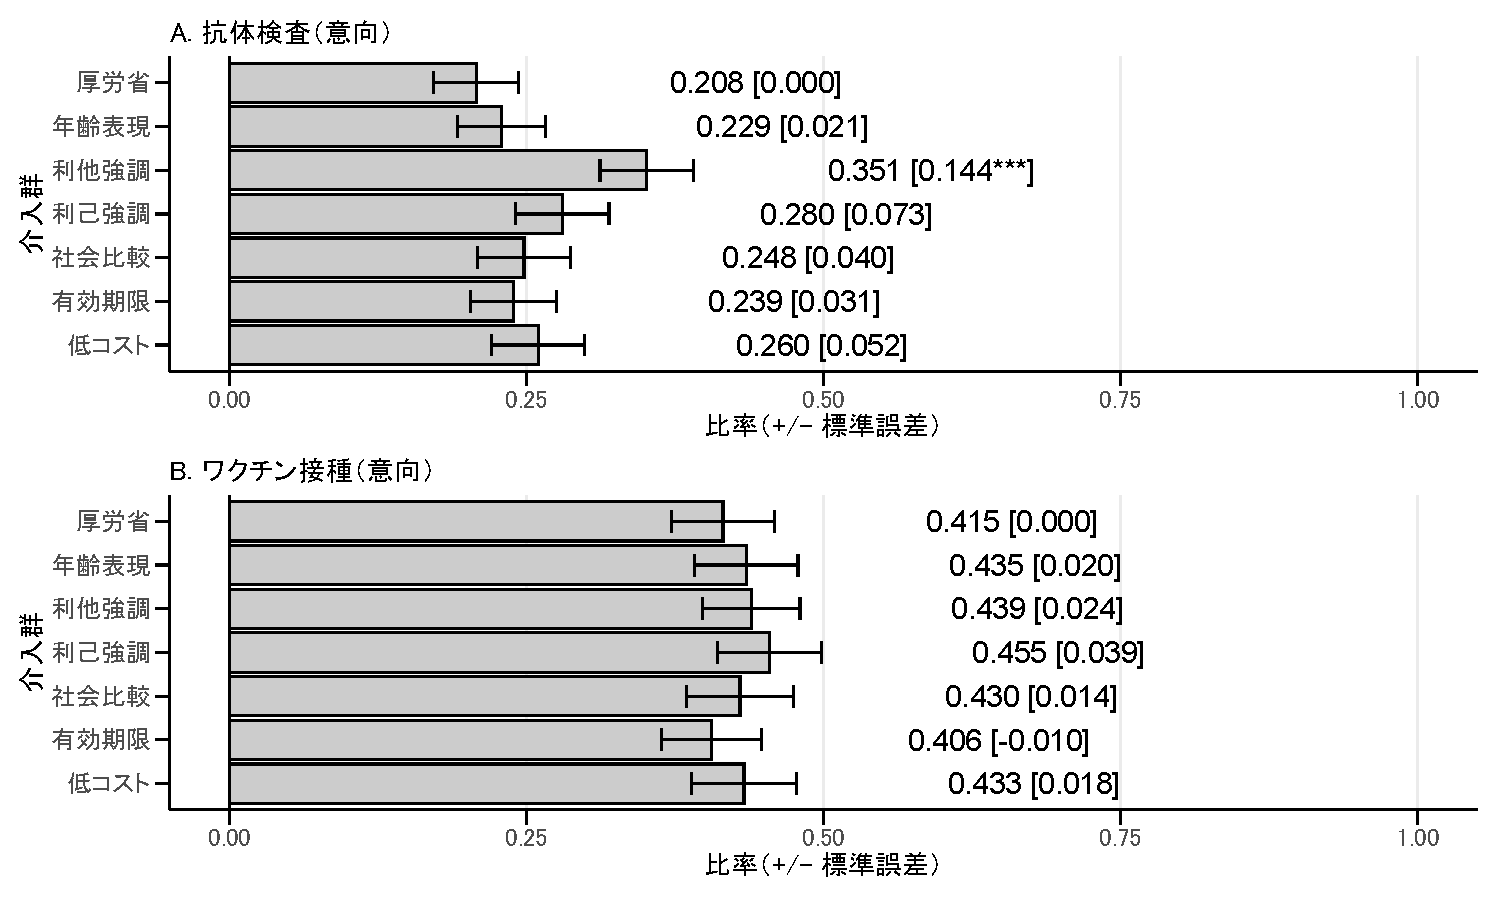
\includegraphics{C:/Users/vge00/Desktop/MHLWRubellaNudge/publish/RIETI/webRCT/webRCT_files/figure-latex/IntentionCoupon1-1} \caption{2019年度クーポン券配布対象者に限定した意向に対するナッジ・メッセージの効果。データソース:Wave 1セレクションデータ。注)図中の数値は各群の比率を示し、角括弧内の数値はナッジ・メッセージの効果の規模(厚労省メッセージ群との差)を示している。効果の統計的な有意性は次の規則に従う:* p < 0.1、** p < 0.05、*** p < 0.01。}\label{fig:IntentionCoupon1}
\end{figure}

図\ref{fig:IntentionCoupon1}は各介入群の抗体検査受検とワクチン接種の意向を示している。
結果として、利他強調メッセージは厚労省メッセージよりも抗体検査受検の意向を高めている。
厚労省メッセージを読んだ人の約20.8\%が抗体検査を受けたいと回答している一方で、
利他強調メッセージを読んだ人の約35.1\%が抗体検査を受けたいと回答している。
したがって、
利他強調メッセージはコントロールよりも約14.3\%ポイント抗体検査の受検意向を引き上げており、
これはt検定より統計的に1\%水準で有意である。
その他のナッジ・メッセージについては、抗体検査を受けたいと答えた人の割合は30\%を下回っていて、
その比率が厚労省メッセージと変わらないという帰無仮説を棄却できない。

図\ref{fig:IntentionCoupon1}のパネルBはワクチン接種の意向を示している。
その結果、
すべての介入群のワクチン接種の意向の比率は40\%から45\%の範囲にあり、
その比率は介入群間で統計的に有意な差とならなかった。
考えられる可能性の一つはワクチン接種の意向の質問文による刺激である。
我々は抗体を持っていないという条件のもとで接種したいかどうかを質問しているので、
質問文がワクチン接種の必要性を強く刺激した可能性がある。

\begin{figure}[t]
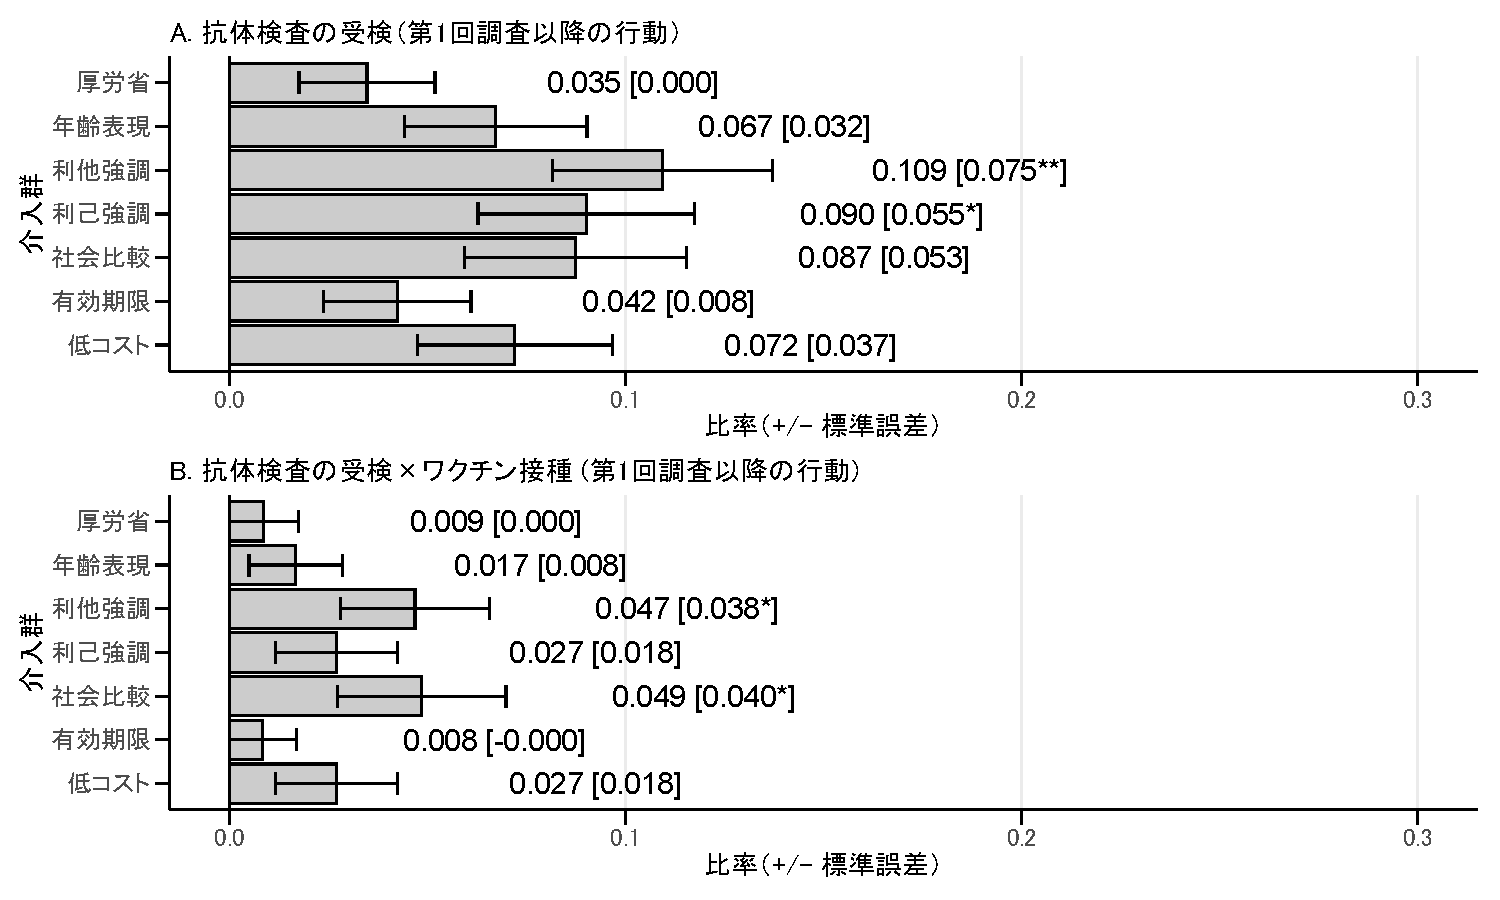
\includegraphics{C:/Users/vge00/Desktop/MHLWRubellaNudge/publish/RIETI/webRCT/webRCT_files/figure-latex/BehaviorCoupon1-1} \caption{2019年度クーポン券配布対象者に限定した行動に対するナッジ・メッセージの効果。データソース:Wave 2セレクションデータ。注)図中の数値は各群の比率を示し、角括弧内の数値はナッジ・メッセージの効果の規模(厚労省メッセージ群との差)を示している。効果の統計的な有意性は次の規則に従う:* p < 0.1、** p < 0.05、*** p < 0.01。}\label{fig:BehaviorCoupon1}
\end{figure}

図\ref{fig:BehaviorCoupon1}のパネルAは各介入群の第1回調査以降の抗体検査受検比率を示している。
結果として、利他強調メッセージと利己強調メッセージでは、厚労省メッセージよりも
第1回調査以降の抗体検査の受検比率が高い。
厚労省メッセージを読んだ人の約3.5\%は第1回調査以降に抗体検査を受検している。
その一方で、利他強調メッセージを読んだ人の約10.9\%と
利己強調メッセージを読んだ人の約9\%は第1回調査以降に抗体検査を受検している。
したがって、利他強調メッセージはコントロールに比べて7.4\%ポイント抗体検査の受検率を引き上げており、
これはt検定より統計的に5\%水準で有意である。
また、利己強調メッセージはコントロールよりも約5.5\%ポイント高く、これはt検定より統計的に10\%水準で有意である。

図\ref{fig:BehaviorCoupon1}のパネルBは
各介入群の第1回調査以降の抗体検査とワクチン接種を両方受けた人の比率(以降、ワクチン接種率と呼ぶ)を示している。
この比率は今回の厚生労働省の政策によって新たに抗体を獲得した人の比率を示すので、
政策効果のアウトカム指標となる。
その結果、利他強調メッセージと社会比較メッセージがワクチン接種を促進していることがわかる。
厚労省メッセージを読んだ人の約0.9\%が抗体検査を受検し、ワクチンを接種している。
その一方で、利他強調メッセージを読んだ人の約4.7\%と
社会比較メッセージを読んだ人の約4.9\%が第1回調査以降に抗体検査を受検し、ワクチンを接種している。
よって、利他強調メッセージは3.8\%ポイントコントロールよりも高く、これはt検定より統計的に10\%水準で有意である。
社会比較メッセージは4\%ポイントコントロールよりも高く、これはt検定より統計的に10\%水準で有意である。

補論\ref{addtab}の表\ref{tab:RegCoupon1}に厚労省メッセージ群を比較対象とした
ナッジ・メッセージの線形確率モデルの推定結果を示した。
ここまでの結果は個人の観察可能な特徴をコントロールしても変化しない。
それに加えて、共変量を制御したモデルを推定すると、
利己強調メッセージは厚労省メッセージよりも抗体検査受検の意向を約9\%ポイント強めていて、
これは統計的に10\%水準で有意である。
さらに、利己強調メッセージと社会比較メッセージは厚労省メッセージと比較して抗体検査の受検行動に
統計的に5\%水準で正の影響を与えている。
効果の規模はそれぞれ6.7\%ポイントと6.5\%ポイントである。

また、効果の規模が最も大きい利他強調メッセージ群を比較対象とした
線形確率モデルの推定結果を補論\ref{addtab}の表\ref{tab:altbase-reg-coupon1}に示した。
その結果、
利己強調メッセージ群の抗体検査受検の意向は利他強調メッセージのそれと統計的に有意な差とならなかった。
さらに、利己強調メッセージと社会比較メッセージの抗体検査の受検比率は
利他強調メッセージのそれと統計的に有意に異ならならなかった。
したがって、効果があった利他強調メッセージとの有意差がないという意味で、
利己強調メッセージは抗体検査受検の意向と行動を促進した可能性があり、
社会比較メッセージは抗体検査の受検を促進した可能性がある。
しかしながら、抗体検査の受検比率の差は検出力を十分に保つほどの大きさではないので、
サンプルサイズを十分に大きくして検証する必要がある。

\begin{table}

\caption{\label{tab:CtabTesterCoupon1}2019年度クーポン券配布対象の抗体検査受検者の動き}
\centering
\resizebox{\linewidth}{!}{
\fontsize{9}{11}\selectfont
\begin{threeparttable}
\begin{tabular}[t]{lccccccc}
\toprule
\multicolumn{2}{c}{ } & \multicolumn{2}{c}{抗体検査の受検} & \multicolumn{2}{c}{抗体検査の結果が陰性} & \multicolumn{2}{c}{陰性かつワクチンを接種} \\
\cmidrule(l{3pt}r{3pt}){3-4} \cmidrule(l{3pt}r{3pt}){5-6} \cmidrule(l{3pt}r{3pt}){7-8}
ナッジ・メッセージ & サンプルサイズ & 人数 & 二群比較のp値 & 人数  & 二群比較のp値 & 人数   & 二群比較のp値\\
\midrule
厚労省 & 115 & 4 & - & 1 & - & 1 & -\\
年齢表現 & 119 & 8 & 0.376 & 2 & 1.000 & 2 & 1.000\\
利他強調 & 128 & 14 & 0.029 & 7 & 0.588 & 6 & 1.000\\
利己強調 & 111 & 10 & 0.102 & 3 & 1.000 & 3 & 1.000\\
社会比較 & 103 & 9 & 0.151 & 5 & 0.559 & 5 & 1.000\\
有効期限 & 118 & 5 & 1.000 & 1 & 1.000 & 1 & 1.000\\
低コスト & 111 & 8 & 0.247 & 5 & 0.545 & 3 & 1.000\\
\bottomrule
\end{tabular}
\begin{tablenotes}
\item 注)二群比較は、厚労省メッセージ群とあるナッジ・メッセージの二群をFisherの正確検定で分析している。抗体検査の受検をアウトカムとするとき、抗体検査の受検者数に群間で差がないという帰無仮説を検定している。抗体検査の陰性者をアウトカムとするとき、抗体検査の受検者の中で陰性者の比率に群間で差がないという帰無仮説を検定している。陰性者のワクチン接種をアウトカムとするとき、陰性者の中でワクチン接種の比率に群間で差がないという帰無仮説を検定している。
\end{tablenotes}
\end{threeparttable}}
\end{table}

利他強調メッセージと社会比較メッセージがワクチン接種を促進した理由は、
厚労省メッセージ群よりも抗体検査の陰性比率が高いことにある。
この点を明らかにするために、
表\ref{tab:CtabTesterCoupon1}に各群の抗体検査受検者の動きを示した。
この表から二つの発見がある。
第一に、利他強調メッセージと低コストメッセージを除くすべての群で、
抗体検査の結果が陰性である人が全員ワクチンを接種している。
たとえば、厚労省メッセージ群では、1人の陰性者がワクチン接種をしているので、
陰性者のワクチン接種比率は100\%である。
ワクチン接種を促進した利他強調メッセージと社会比較メッセージの
陰性者のワクチン接種比率はそれぞれ
86\%(\(=6/7\))と100\%(\(=5/5\))である。

第二に、各群の抗体検査の陰性比率は20\%から62.5\%の範囲にある。
たとえば、厚労省メッセージ群では、4人の抗体検査受検者のうち、
1人が陰性であったので、陰性比率は約25\%である。
ワクチン接種を促進した利他強調メッセージと社会比較メッセージの陰性比率はそれぞれ
50\%(\(=7/14\))と56\%(\(=5/9\))である。
したがって、厚労省メッセージと比較して、
利他強調メッセージと社会比較メッセージはワクチンを接種するべき人が多くいたので、
これらのメッセージがワクチン接種に対して正の効果があった。
また、利他強調メッセージ群の陰性者のワクチン接種率が100\%を下回っているので、
ワクチン接種に対する社会比較メッセージの効果の規模(4\%ポイント)が
利他強調メッセージ(3.8\%ポイント)より若干大きくなった。

ただし、利他強調メッセージと社会比較メッセージの抗体検査の陰性比率が
厚労省メッセージより高いという発見は偶然である可能性が高い。
我々はあるナッジ・メッセージ群と厚労省メッセージ群の抗体検査受検者に限定して、
陰性者の数が群間で異ならないという帰無仮説を
フィッシャーの正確検定で検証し、
そのp値を表\ref{tab:CtabTesterCoupon1}の第6列に示した。
すべてのナッジ・メッセージ群において、
陰性者の数が厚労省のそれと異ならないという帰無仮説を棄却できなかった。
よって、我々のデータでは陰性比率が各群で異なっているが、
母集団では陰性比率は群間で差がない\footnote{陰性者のワクチン接種比率についても同様の結果が得られた。
  すなわち、利他強調メッセージと厚労省メッセージで、
  陰性者のワクチン接種の数に差がない
  (表\ref{tab:CtabTesterCoupon1}の第8列より、p値は1)。}。

また、介入に関わらず抗体検査の結果が陰性である人のほとんどがワクチンを接種しているという事実は、
抗体検査の受検率を高めることが政策的に重要であることを示唆している。
抗体保有率を高めるための政策介入は二種類が考えられる。
第一に、単純に抗体検査の受検者を増やす政策である。
第二に、抗体検査の結果が陰性である人がワクチンを接種することを促進する政策である。
今回のランダム化比較試験は後者の介入をしていないにも関わらず、
ほとんどの陰性者がワクチンを接種している\footnote{介入群ごとにデータを分割しない場合の陰性者のワクチン接種比率は
  87.5\%
  であった。また、1000個のブートストラップ標本で構築した95\%信頼区間は100\%を含んでいる
  (95\%信頼区間は、
  {[}75.0\%, 100.0\%{]}
  )。}。
これは陰性者のワクチン接種を促進する政策よりも抗体検査の受検を促進する政策の方が
効率的に抗体保有率を高められることを示唆している。
このとき、抗体を保有していない人に抗体検査を受検させるような政策を用いることで、
より政策目標を達成できる\footnote{陰性であるにも関わらず抗体検査を受検していない人がいるはずなので、
  陰性者の抗体検査受検率をデータから直接復元することはできない。
  しかしながら、ベイズ定理を用いて、間接的に推定することができる。
  それを示すために、陰性という事象\(A\)と抗体検査の受検という事象\(B\)の二つの事象を考える。
  このとき、抗体検査の受検比率は\(P(B)\)、抗体検査受検者の陰性比率は\(P(A|B)\)で表すことができ、
  これらの値はデータから直接推定できる。
  ベイズの定理より、抗体検査受検者の陰性比率は
  \[ P(A|B) = \frac{P(B|A) \cdot P(A)}{P(B)} \]
  と定義できる。
  ここで、\(P(A)\)は陰性比率であり、
  これは第\ref{background}節で示したNIIDのデータより0.2となる。
  確率\(P(B|A)\)は陰性者で条件づけた抗体検査の受検比率であり、我々の関心のあるパラメータである。
  よって、陰性者の抗体検査の受検比率は
  \[ \hat{P}(B|A) = \frac{\hat{P}(A|B) \cdot \hat{P}(B)}{0.2} \]
  で計算できる。
  介入群でサンプルを分割しなかった場合、
  \(\hat{P}(A|B) = 0.413\)と\(\hat{P}(B) = 0.072\)なので、
  \(\hat{P}(B|A) = 0.149\)となる(1000個のブートストラップ標本で構築した95\%信頼区間は
  {[}0.099, 0.205{]} )。
  さらに、陰性であるかどうかによって抗体検査の受検にセレクションが生じているかどうかを
  検証するために、陰性という事象と抗体検査の受検という事象が独立であるという帰無仮説を検定した。
  \(\hat{P}(B|A) - \hat{P}(B)\)の95\%信頼区間にゼロが含まれていないとき、
  我々は帰無仮説を5\%有意水準で棄却できる。
  \(\hat{P}(B|A) - \hat{P}(B)\)の95\%信頼区間は
  {[}0.034, 0.128{]}
  なので、我々は帰無仮説を棄却できる。
  言い換えれば、抗体を保有していない人が抗体検査を受検している傾向にある。}。

\hypertarget{econvalue}{%
\subsection{ナッジ・メッセージの金銭的価値}\label{econvalue}}

\begin{figure}[t]
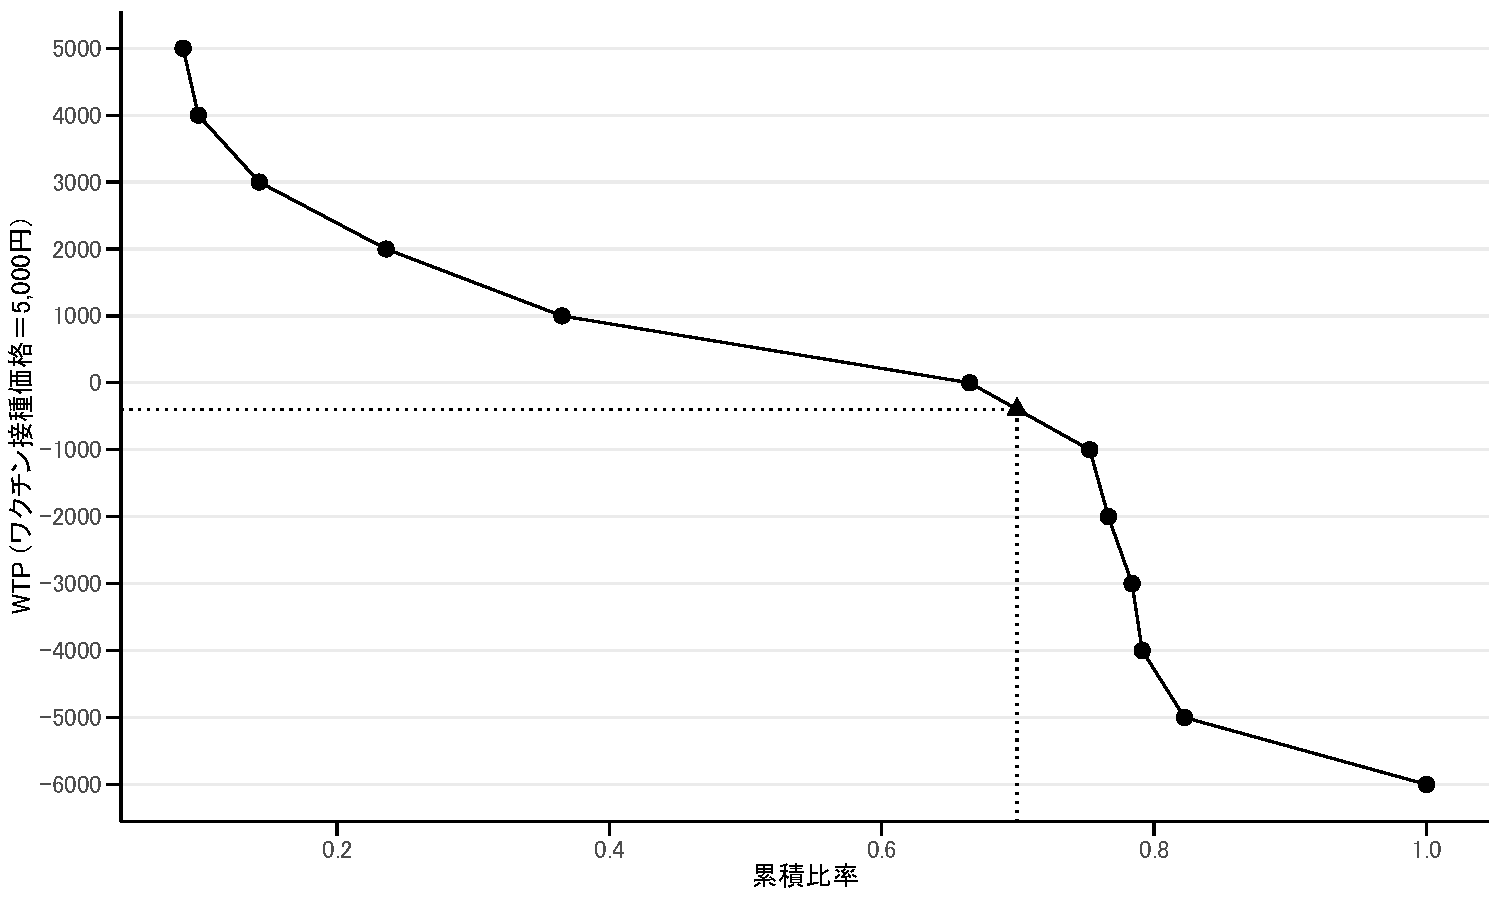
\includegraphics{C:/Users/vge00/Desktop/MHLWRubellaNudge/publish/RIETI/webRCT/webRCT_files/figure-latex/demandVaccine-1} \caption{2019年度クーポン券配布対象者の風しんワクチンの需要曲線。データソース:Wave 1セレクションデータ。注)黒の三角はワクチン接種費用が無料であるときの接種割合と厚労省メッセージの抗体検査受検率を合計した割合と、それに対応するWTPを示している。}\label{fig:demandVaccine}
\end{figure}

2019年度のクーポン券送付者におけるナッジ・メッセージの効果を金銭的な価値で評価することを試みる。
そのために、第1回調査のナッジ・メッセージを示す前の質問票Aで調査したワクチン接種の支払意思額を用いる。
ワクチンの価格は5000円と仮定して、我々は、自治体の補助金額が\(s_j\)のとき、ワクチン接種をするかどうかを調査した。
補助金額は\(s_j \in \{0, 1000, 2000, \ldots, 10000\}\)とした。
回答者\(i\)が接種すると回答した最低の補助金額を\(s_i^{\text{min}}\)とする。
回答者\(i\)が接種しないと回答した最高の補助金額を\(s_i^{\text{max}}\)とする。
このとき、回答者\(i\)の支払意思額は
\([5000 - s_i^{\text{min}}, 5000 - s_i^{\text{max}})\)の範囲内で識別される\footnote{回答者がすべての補助金額\(s_j\)のときの接種しないと回答したならば、\(s_i^{\text{max}} = 10000\)である。しかしながら、\(s_i^{\text{min}}\)はデータで定義できない。そこで、\(s_i^{\text{min}} = 11000\)と仮定した。ただし、後に示すが、この仮定はナッジ・メッセージの金銭的価値に影響を与えない。}。
したがって、追加の仮定を置かない限り、ワクチン接種の需要曲線はステップワイズな曲線となり、
メッセージの金銭的価値は範囲で得られる。

メッセージの金銭的価値を点推定するために、
我々は支払意思額が\([5000 - s_i^{\text{min}}, 5000 - s_i^{\text{max}})\)の範囲で識別されるとき、
真の支払意思額はその範囲内で一様に分布することを仮定する。
このとき、ステップワイズなワクチン接種の需要曲線は線型補間で表される。
図\ref{fig:demandVaccine}はこの仮定のもとで、2019年度に自動的にクーポン券を受け取る人に限定した
風しんワクチン接種の需要曲線である。
我々はこの需要曲線を用いて、メッセージの金銭的価値を算出する。

\begin{table}

\caption{\label{tab:econvalue}ナッジ・メッセージの金銭的価値の推定}
\centering
\resizebox{\linewidth}{!}{
\fontsize{9}{11}\selectfont
\begin{threeparttable}
\begin{tabular}[t]{lcccccc}
\toprule
\multicolumn{3}{c}{ } & \multicolumn{2}{c}{金銭的価値(日本円)} & \multicolumn{2}{c}{金銭的価値(米ドル)} \\
\cmidrule(l{3pt}r{3pt}){4-5} \cmidrule(l{3pt}r{3pt}){6-7}
ナッジ・メッセージ & 効果の規模 & ベースライン+効果の規模 & 一人当たり & 総額 & 一人当たり  & 総額 \\
\midrule
年齢表現 & 0.032 & 0.732 & 367.854 & 1.946 & 3.344 & 17.690\\
利他強調 & 0.075 & 0.774 & 2037.553 & 10.779 & 18.523 & 97.988\\
利己強調 & 0.055 & 0.755 & 744.045 & 3.936 & 6.764 & 35.782\\
社会比較 & 0.053 & 0.752 & 596.335 & 3.155 & 5.421 & 28.678\\
有効期限 & 0.008 & 0.707 & 86.059 & 0.455 & 0.782 & 4.139\\
低コスト & 0.037 & 0.737 & 422.789 & 2.237 & 3.844 & 20.332\\
\bottomrule
\end{tabular}
\begin{tablenotes}
\item 注) 抗体検査の受検に対するナッジ・メッセージの効果を効果の規模として用いた。 ベースラインはワクチン接種費用が無料であるときの接種割合と 厚労省メッセージの抗体検査受検率を合計した割合である。 金銭的価値は一人当たりの価値と それに2020年1月時点でワクチンクーポン券を利用していない人数(529万人)をかけた 総額を示している。 また、金銭的価値は日本円と米ドルで示した(1ドル=110円)。 一人当たりの金銭的価値の単位はそれぞれ1円と1ドルである。 総額で示した金銭的価値の単位はそれぞれ10億円と100万ドルである。
\end{tablenotes}
\end{threeparttable}}
\end{table}

ナッジ・メッセージの金銭的な価値を次のように計算する。
はじめに、ベースラインの接種割合を決める。
図\ref{fig:demandVaccine}の需要曲線は無料クーポンが発行される人に限定しているので、
ワクチンの供給曲線はゼロで水平である。
このときの接種割合は約66.5\%である。
ベースラインの接種割合はこの割合に厚労省メッセージの抗体検査受検率を足したものとする\footnote{抗体検査の結果が陰性である人のほとんどはワクチンを接種しているので、
  抗体検査の受検率をワクチン接種率として用いる。}。
ベースラインの接種割合は約70\%であり、対応する支払意思額は約-394円である。

次に、接種割合をベースラインの均衡点からナッジ・メッセージの効果分だけ増やすとき、
需要曲線上で対応する支払意思額を見つける。
その支払意思額はナッジ・メッセージの効果量だけ増やすのに必要な自治体の追加的な補助金額であり、
それがナッジ・メッセージの一人当たりの金銭的価値である。
たとえば、ベースラインの均衡点の接種割合とナッジ・メッセージの効果の和が0.8であるとき、
需要曲線上で対応する支払意思額は約-4280円である。
すなわち、ナッジ・メッセージの効果量分だけ接種割合を増やすために、
自治体は一人当たり約3886(\(=4280-394\))円の追加的な補助金を支払う必要がある。

我々は抗体検査受検に対するナッジ・メッセージの効果を用いる。
表\ref{tab:CtabTesterCoupon1}で示したように、
抗体検査の結果が陰性である人のほとんどはワクチンを接種している。
したがって、抗体検査受検に対するナッジ・メッセージの効果をワクチン接種に対する効果とみなせる。

表\ref{tab:econvalue}はメッセージの金銭的価値の試算結果である。
第2列は図\ref{fig:BehaviorCoupon1}のパネルAで示したメッセージの効果を示している。
第3列はベースラインの均衡点の接種割合からメッセージの効果量分だけ増やしたときの接種割合を示している。
第4列はメッセージの一人当たりの金銭的価値である。
この金銭的価値をアメリカドルに換算した結果を第6列に示している。
抗体検査の受検を促進した利他強調メッセージの一人当たりの金銭的価値は約2000円(約18ドル)である。

また、メッセージ自体の金銭的価値の総額は一人当たりの金銭的価値と
2019年度に発行されたクーポン券をまだ利用していない人数の積で得られる。
厚生労働省より、2019年度にクーポン券が発行されたにもかかわらず、
1月時点で抗体検査のクーポン券を利用していない人は約529万人である。
表\ref{tab:econvalue}の第5列はメッセージの金銭的価値の総額を示している。
第7列はそれをアメリカドルに換算した結果を示している。
利他強調メッセージの金銭的価値の総額は約100億円である。

\hypertarget{coupon0}{%
\subsection{2019年度クーポン券送付対象外の男性に限定したナッジ・メッセージの効果}\label{coupon0}}

次に、2019年度には、クーポン券の送付対象ではないが、
オンデマンドでクーポン券を受け取れる人に限定して、
ナッジ・メッセージの効果を推定する。

\begin{figure}[t]
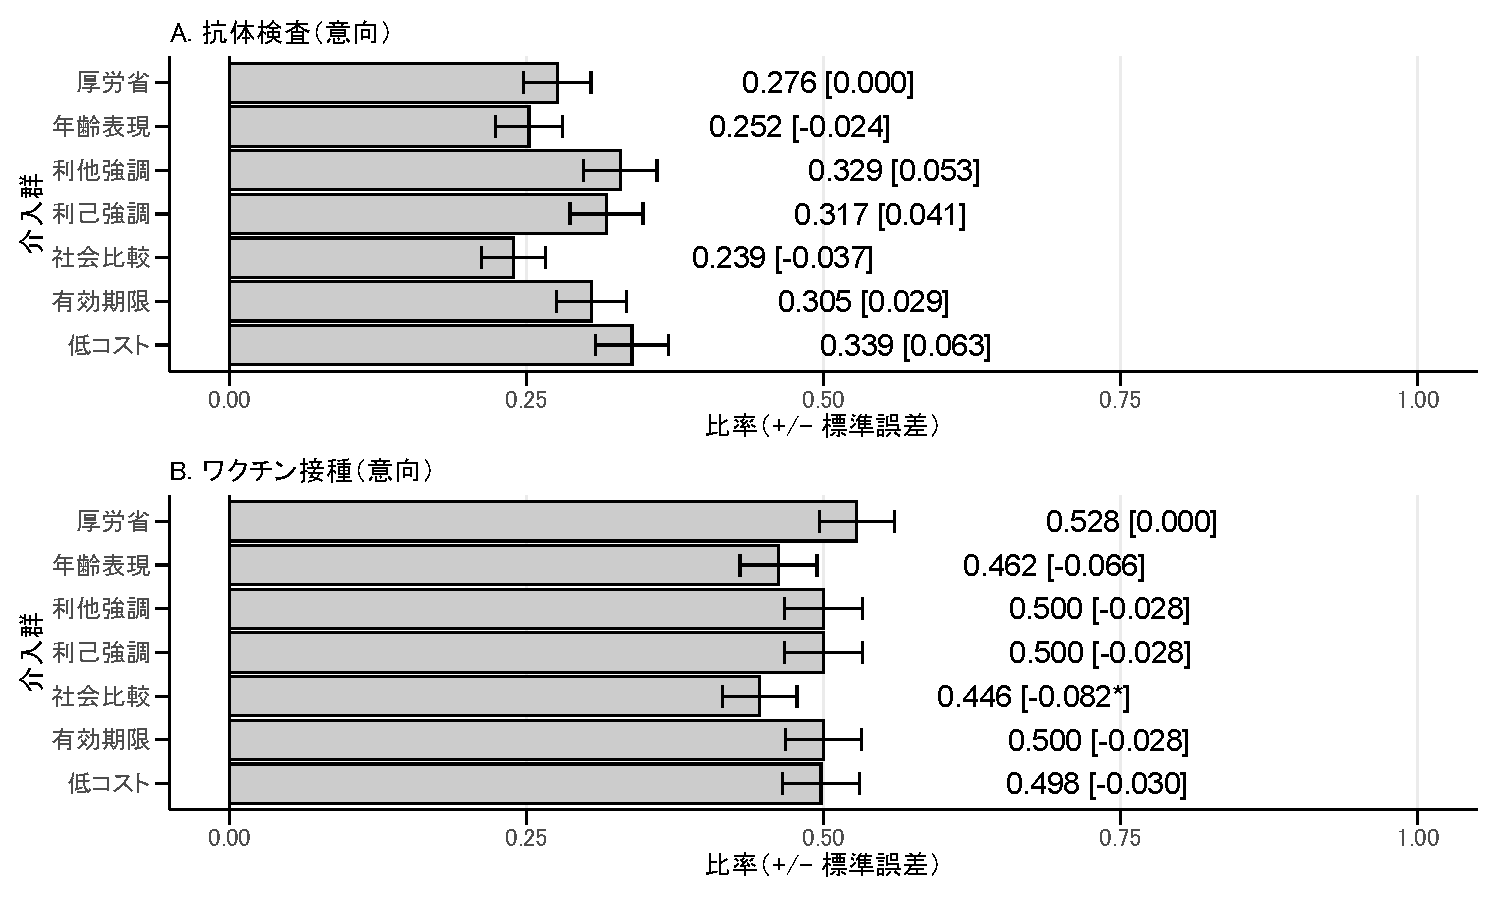
\includegraphics{C:/Users/vge00/Desktop/MHLWRubellaNudge/publish/RIETI/webRCT/webRCT_files/figure-latex/IntentionCoupon0-1} \caption{2019年度クーポン券配布対象外の男性に限定した意向に対するナッジ・メッセージの効果。データソース:Wave 1セレクションデータ。注)図中の数値は各群の比率を示し、角括弧内の数値はナッジ・メッセージの効果の規模(厚労省メッセージ群との差)を示している。効果の統計的な有意性は次の規則に従う:* p < 0.1、** p < 0.05、*** p < 0.01。}\label{fig:IntentionCoupon0}
\end{figure}

図\ref{fig:IntentionCoupon0}は介入群ごとの抗体検査受検とワクチン接種の意向の比率を示している。
図\ref{fig:IntentionCoupon1}と同様に、すべての介入群について、
抗体検査受検の意向の比率はワクチン接種の意向の比率より低い。
2019年度にクーポン券が送付されない人に対しても、
ワクチン接種の意向の質問文は抗体検査が陰性だったという条件付であることに注意して解釈すべきである。

また、社会比較メッセージは抗体検査受検の意向に対して統計的に有意な効果を持っていないが、
ワクチン接種の意向に対して負の効果を持っている。
厚労省メッセージを読んだ人の抗体検査受検とワクチン接種の意向の比率はそれぞれ約27.6\%と約52.8\%である。
それに対して、社会比較メッセージを読んだ人の抗体検査受検とワクチン接種の意向の比率はそれぞれ
約23.9\%と約44.6\%である。
したがって、社会比較メッセージの抗体検査受検の意向に対する効果は約-3.7\%ポイントであり、
これは統計的に有意な効果ではない。
しかしながら、社会比較メッセージのワクチン接種の意向に対する効果は約-8.2\%ポイントであり、
これは統計的に10\%水準で有意である。

この負の効果の原因の一つとして、ワクチン接種のただ乗りが挙げられる。
社会比較メッセージは「5人に1人が抗体を持っていない」ことを強調している。
裏返せば、5人に4人が抗体を持っているということである。
このメッセージを読んだ人は、仮に風しんの抗体を保有していないとしても、
全体の80\%が抗体を持っているので、自身が感染する機会は少ないと考えたのかもしれない。
クーポン券がない場合、
この信念がワクチンを接種することの価値を低め、ワクチン接種の意向の比率をコントロールよりも下げた可能性がある。

\begin{figure}[t]
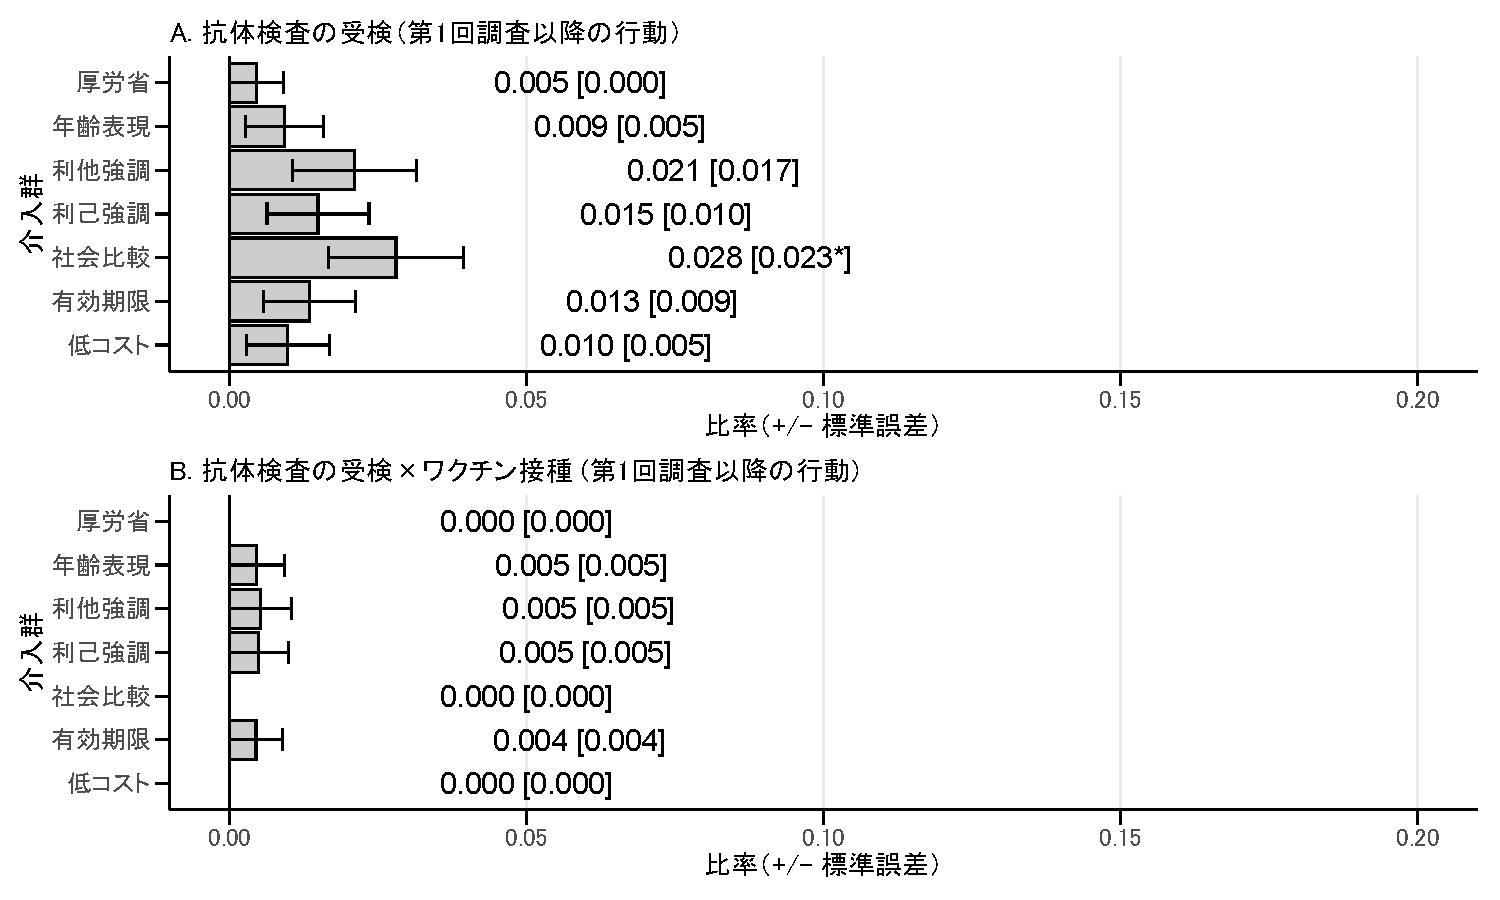
\includegraphics{C:/Users/vge00/Desktop/MHLWRubellaNudge/publish/RIETI/webRCT/webRCT_files/figure-latex/BehaviorCoupon0-1} \caption{2019年度クーポン券配布対象外の男性に限定した行動に対するナッジ・メッセージの効果。データソース:Wave 2セレクションデータ。注)図中の数値は各群の比率を示し、角括弧内の数値はナッジ・メッセージの効果の規模(厚労省メッセージ群との差)を示している。効果の統計的な有意性は次の規則に従う:* p < 0.1、** p < 0.05、*** p < 0.01。}\label{fig:BehaviorCoupon0}
\end{figure}

図\ref{fig:BehaviorCoupon0}は各介入群の第1回調査以降の抗体検査受検比率と
第1回調査以降のワクチン接種比率である。
社会比較メッセージが厚労省メッセージよりも第1回調査以降の抗体検査の受検を促進しているが、
抗体検査とワクチン接種の両方を促進していない。
厚労省メッセージを読んだ人の約0.5\%が第1回調査以降に抗体検査を受検したが、
誰もワクチン接種をしていない。
また、社会比較メッセージを読んだ人の約2.8\%が第1回調査以降に抗体検査を受検したが、
誰もワクチン接種をしていない。
よって、社会比較メッセージの抗体検査受検に対する効果は約2.3\%ポイントであり、
これは統計的に10\%水準で有意である。
しかしながら、抗体検査とワクチン接種の両方に対する効果はゼロである。

ここまでの結果は表\ref{tab:covlist}で示した個人の観察可能な特徴をコントロールしても変化しない。
表\ref{tab:RegCoupon0}はナッジ・メッセージの線形確率モデルの推定結果である。
奇数列はナッジ・メッセージのダミー変数のみを説明変数に加えているので、
これらの結果は二群間のt検定の結果
(図\ref{fig:IntentionCoupon0}と図\ref{fig:BehaviorCoupon0})に対応している。
偶数列はナッジ・メッセージのダミー変数に加えて、表\ref{tab:covlist}の変数を説明変数に加えている。
列(4)は、これまでの結果に加えて、
年齢表現メッセージが抗体検査の受検に負の効果を持っていることを示しており、
これは統計的に5\%水準で有意である。

\begin{table}

\caption{\label{tab:CtabTesterCoupon0}2019年度クーポン券配布対象外の抗体検査受検者の動き}
\centering
\resizebox{\linewidth}{!}{
\fontsize{9}{11}\selectfont
\begin{threeparttable}
\begin{tabular}[t]{lccccccc}
\toprule
\multicolumn{2}{c}{ } & \multicolumn{2}{c}{抗体検査の受検} & \multicolumn{2}{c}{抗体検査の結果が陰性} & \multicolumn{2}{c}{陰性かつワクチンを接種} \\
\cmidrule(l{3pt}r{3pt}){3-4} \cmidrule(l{3pt}r{3pt}){5-6} \cmidrule(l{3pt}r{3pt}){7-8}
ナッジ・メッセージ & サンプルサイズ & 人数 & 二群比較のp値 & 人数  & 二群比較のp値 & 人数   & 二群比較のp値\\
\midrule
厚労省 & 220 & 1 & - & 0 & - & 0 & -\\
年齢表現 & 216 & 2 & 0.621 & 2 & 0.333 & 1 & -\\
利他強調 & 190 & 4 & 0.187 & 1 & 1.000 & 1 & -\\
利己強調 & 201 & 3 & 0.352 & 1 & 1.000 & 1 & -\\
社会比較 & 214 & 6 & 0.065 & 1 & 1.000 & 0 & -\\
有効期限 & 223 & 3 & 0.623 & 1 & 1.000 & 1 & -\\
低コスト & 203 & 2 & 0.610 & 0 & 1.000 & 0 & -\\
\bottomrule
\end{tabular}
\begin{tablenotes}
\item 注)二群比較は、厚労省メッセージ群とあるナッジ・メッセージの二群をFisherの正確検定で分析している。抗体検査の受検をアウトカムとするとき、抗体検査の受検者数に群間で差がないという帰無仮説を検定している。抗体検査の陰性者をアウトカムとするとき、抗体検査の受検者の中で陰性者の比率に群間で差がないという帰無仮説を検定している。陰性者のワクチン接種をアウトカムとするとき、陰性者の中でワクチン接種の比率に群間で差がないという帰無仮説を検定している。
\end{tablenotes}
\end{threeparttable}}
\end{table}

第\ref{coupon1}節で示したように、
ワクチン接種比率が抗体検査の受検比率より低い原因は、
抗体検査の陰性比率が低いことにある。
表\ref{tab:CtabTesterCoupon0}に抗体検査受検者の動きを示した。
各群の抗体検査の陰性比率は0\%から100\%の範囲にある。
とくに、厚労省メッセージの抗体検査の陰性比率は0\%(\(=0/1\))である。
抗体検査を促進した社会比較メッセージの陰性比率は17\%(\(=1/6\))である。
しかしながら、フィッシャーの正確検定より、
これらの二群の陰性比率の差は統計的に有意でない
(第6列より、p値は1)。

また、第\ref{coupon1}節と同様に、
抗体検査の結果が陰性である人のほとんどがワクチンを接種していることも明らかになった。
厚労省メッセージ群と低コストメッセージ群では、陰性者がいない。
残った介入群のうち、社会比較メッセージ群を除くすべての群において、
抗体検査の結果が陰性である人は全員ワクチンを接種していた。

\hypertarget{conclusion}{%
\section{議論と結論}\label{conclusion}}

本研究は、オンラインサーベイによるランダム化比較試験(RCT)を用いて、
風しんワクチンの接種を促進するためにどのようなナッジ・メッセージが有効であるかを明らかにした。
主な結果は以下の三つにまとめられる。
第一に、2019年度にクーポン券送付対象の年齢の男性のみに利他強調メッセージが抗体検査の受検を7.5\%ポイント促進した。
このメッセージの効果を金銭的価値で評価すると、一人当たりの金銭的価値は約2000円(約18ドル)であり、
その総額は約100億円(約9,700万ドル)である。
この効果は個人の観察可能な特徴に対して頑健であり、
サンプルサイズが小さいことを考慮したフィッシャーの正確検定でも、
この効果は5\%水準で有意である(表\ref{tab:CtabTesterCoupon1}の第4列)。
また、利己強調メッセージや社会比較メッセージの抗体検査の受検比率は利他強調メッセージ群のそれと有意な差ではない。
この意味で、二つのメッセージも抗体検査の受検を促進した可能性がある。
しかしながら、抗体検査の受検比率の差は検出力を十分に保てるほどの大きさではないので、
サンプルサイズを増やした再検証が必要である。

第二に、介入群に関わらず、抗体検査の結果が陰性である人のほとんどはワクチンを接種していた。
これは、抗体保有率を高めるために、陰性である人のワクチン接種率を高めるような政策ではなく、
抗体検査の受検比率を高めるような政策の方が効率的であることを示唆している。
したがって、利他強調メッセージは抗体保有率を高めるためのナッジ・メッセージとして有効である。

第三に、2019年度にクーポン券がオンデマンドでしか送付されない年齢層の男性に対してナッジ・メッセージは機能しなかった。
考えられる可能性が二つある。
第一に、2019年度にクーポン券の送付対象ではない男性は厚生労働省の無料クーポン券制度を認知していないという点である。
第1回調査の調査票A(ナッジ・メッセージを示す前の調査)で、我々は厚生労働省のクーポン券制度の認知度を調査した。
その結果、2019年度にクーポン券の送付対象ではない年齢層の男性の約
77.5\%
が厚生労働省のクーポン券制度を知らなかった。
仮にナッジ・メッセージを読んで、風しんの抗体検査やワクチン接種を受ける必要性を理解したとしても、
クーポン券の存在を知らない人はそれらの予防行動を自費で受けないといけないと考えている。
ナッジ・メッセージは予防行動のコストを上回るほどその価値を高められなかったのかもしれない。
第二に、クーポン券制度を認知していて無料接種対象の年齢であったとしても、
2019年度にクーポン券の送付対象ではない年齢の男性は自治体にクーポン券を発行してもらうように依頼する必要があるという点である。
クーポン券制度を認知している男性が無料で抗体検査やワクチン接種を受けられることを知っていても、
クーポン券の発行の手続き自体にコストが伴う。
したがって、ナッジ・メッセージはクーポン券の発行の手続きのコストを上回るほどその価値を高められなかったのかもしれない。

分析結果について考慮すべき点が一つある。
ナッジ・メッセージの行動に対する効果を推定するとき、
我々はWave 2で前回のアンケート調査以前に抗体検査もしくはワクチン接種を受けたと回答した人を除いている。
しかしながら、この回答は想起バイアスを伴っている可能性がある。
もしそうならば、サンプルセレクションに想起バイアスが伴うので、
Wave 2でWave 1以前に抗体検査もしくはワクチン接種を受けたという人を除くべきではない。
したがって、想起バイアスを想定した分析では、Wave 1で過去に抗体検査もしくはワクチン接種を受けたと回答した人を除いたサブサンプルと、
抗体検査やワクチン接種を受けた時期に基づかないアウトカム変数を用いるべきである。
想起バイアスを想定した分析では、
効果・統計的な有意性・効果の金銭的価値は大きく異なるものの、
利他強調メッセージが抗体検査の受検を促進していることを確認している
(詳細な結果は補論Bに示した)。

最後に、新たなナッジ政策の方向性を議論しておく。
第一に、クーポン券を得ることで無料で抗体検査やワクチン接種を受けられること、
そして、その手続きの方法を分かりやすく伝えるようなナッジ・メッセージは有効かもしれない。
2019年度にクーポン券が配布されなかった男性に対して、
我々が開発したナッジ・メッセージは有効ではなかった。
先に述べたように、その原因はそもそもクーポン券制度の存在を知らなかった、
もしくはクーポン券の発行の手続きのコストが高いことにあると考えられる。
こうした問題点を解消するようなナッジ政策は有効だろう。
ただし、これは今回の厚生労働省の風しん対策特有の問題であることに注意したい。
第二に、実際は抗体を保有していないが、風しんに感染した経験があると思っていたり、ワクチンを接種したと思っていて、
抗体を保有していると誤って信じているような人の抗体検査の受検を促進することである。
抗体保有の誤った信念を正すようなナッジ政策がより効率的に政策目標を達成できるだろう。
このようなナッジ政策の効果検証が今後の研究課題となる。

\newpage

\hypertarget{ux53c2ux8003ux6587ux732e}{%
\section*{参考文献}\label{ux53c2ux8003ux6587ux732e}}
\addcontentsline{toc}{section}{参考文献}

\hypertarget{refs}{}
\begin{CSLReferences}{1}{0}
\leavevmode\vadjust pre{\hypertarget{ref-Banerjee2010}{}}%
Banerjee, A.V., Duflo, E., Glennerster, R., Kothari, D., 2010. Improving immunisation coverage in rural {India}: Clustered randomised controlled evaluation of immunisation campaigns with and without incentives. BMJ 340, c2220--c2220. doi:\href{https://doi.org/10.1136/bmj.c2220}{10.1136/bmj.c2220}

\leavevmode\vadjust pre{\hypertarget{ref-Barber2022}{}}%
Barber, A., West, J., 2022. Conditional cash lotteries increase {COVID-19} vaccination rates. Journal of Health Economics 81, 102578. doi:\href{https://doi.org/10.1016/j.jhealeco.2021.102578}{10.1016/j.jhealeco.2021.102578}

\leavevmode\vadjust pre{\hypertarget{ref-Barham2009}{}}%
Barham, T., Maluccio, J.A., 2009. Eradicating diseases: {The} effect of conditional cash transfers on vaccination coverage in rural {Nicaragua}. Journal of Health Economics 28, 611--621. doi:\href{https://doi.org/10.1016/j.jhealeco.2008.12.010}{10.1016/j.jhealeco.2008.12.010}

\leavevmode\vadjust pre{\hypertarget{ref-Benartzi2017}{}}%
Benartzi, S., Beshears, J., Milkman, K.L., Sunstein, C.R., Thaler, R.H., Shankar, M., Tucker-Ray, W., Congdon, W.J., Galing, S., 2017. Should {Governments Invest More} in {Nudging}? Psychol Sci 28, 1041--1055. doi:\href{https://doi.org/10.1177/0956797617702501}{10.1177/0956797617702501}

\leavevmode\vadjust pre{\hypertarget{ref-Brehm2021}{}}%
Brehm, M., Brehm, P., Saavedra, M., 2021. The {Ohio Vaccine Lottery} and {Starting Vaccination Rates}. American Journal of Health Economics. doi:\href{https://doi.org/10.1086/718512}{10.1086/718512}

\leavevmode\vadjust pre{\hypertarget{ref-Bronchetti2015}{}}%
Bronchetti, E.T., Huffman, D.B., Magenheim, E., 2015. Attention, intentions, and follow-through in preventive health behavior: {Field} experimental evidence on flu vaccination. Journal of Economic Behavior \& Organization 116, 270--291. doi:\href{https://doi.org/10.1016/j.jebo.2015.04.003}{10.1016/j.jebo.2015.04.003}

\leavevmode\vadjust pre{\hypertarget{ref-Bursztyn2019}{}}%
Bursztyn, L., Fiorin, S., Gottlieb, D., Kanz, M., 2019. Moral {Incentives} in {Credit Card Debt Repayment}: {Evidence} from a {Field Experiment}. Journal of Political Economy 127, 1641--1683. doi:\href{https://doi.org/10.1086/701605}{10.1086/701605}

\leavevmode\vadjust pre{\hypertarget{ref-Campos-Mercade2021}{}}%
Campos-Mercade, P., Meier, A.N., Schneider, F.H., Meier, S., Pope, D., Wengström, E., 2021. Monetary incentives increase {COVID-19} vaccinations. Science eabm0475. doi:\href{https://doi.org/10.1126/science.abm0475}{10.1126/science.abm0475}

\leavevmode\vadjust pre{\hypertarget{ref-Chapman2010}{}}%
Chapman, G.B., Li, M., Colby, H., Yoon, H., 2010. Opting {In} vs {Opting Out} of {Influenza Vaccination}. JAMA 304, 43. doi:\href{https://doi.org/10.1001/jama.2010.892}{10.1001/jama.2010.892}

\leavevmode\vadjust pre{\hypertarget{ref-Chetty2009}{}}%
Chetty, R., Looney, A., Kroft, K., 2009. Salience and {Taxation}: {Theory} and {Evidence}. American Economic Review 99, 1145--1177. doi:\href{https://doi.org/10.1257/aer.99.4.1145}{10.1257/aer.99.4.1145}

\leavevmode\vadjust pre{\hypertarget{ref-Dai2021}{}}%
Dai, H., Saccardo, S., Han, M.A., Roh, L., Raja, N., Vangala, S., Modi, H., Pandya, S., Sloyan, M., Croymans, D.M., 2021. Behavioural nudges increase {COVID-19} vaccinations. Nature 597, 404--409. doi:\href{https://doi.org/10.1038/s41586-021-03843-2}{10.1038/s41586-021-03843-2}

\leavevmode\vadjust pre{\hypertarget{ref-DellaVigna2020}{}}%
DellaVigna, S., Linos, E., 2020. {RCTs} to {Scale}: {Comprehensive Evidence} from {Two Nudge Units} (No. w27594). {National Bureau of Economic Research}, {Cambridge, MA}. doi:\href{https://doi.org/10.3386/w27594}{10.3386/w27594}

\leavevmode\vadjust pre{\hypertarget{ref-Hallsworth2017}{}}%
Hallsworth, M., List, J.A., Metcalfe, R.D., Vlaev, I., 2017. The behavioralist as tax collector: {Using} natural field experiments to enhance tax compliance. Journal of Public Economics 148, 14--31. doi:\href{https://doi.org/10.1016/j.jpubeco.2017.02.003}{10.1016/j.jpubeco.2017.02.003}

\leavevmode\vadjust pre{\hypertarget{ref-Ibuka2014}{}}%
Ibuka, Y., Li, M., Vietri, J., Chapman, G.B., Galvani, A.P., 2014. Free-{Riding Behavior} in {Vaccination Decisions}: {An Experimental Study}. PLoS ONE 9, e87164. doi:\href{https://doi.org/10.1371/journal.pone.0087164}{10.1371/journal.pone.0087164}

\leavevmode\vadjust pre{\hypertarget{ref-Kinoshita2016}{}}%
Kinoshita, R., Nishiura, H., 2016. Assessing herd immunity against rubella in {Japan}: A retrospective seroepidemiological analysis of age-dependent transmission dynamics. BMJ Open 6, e009928. doi:\href{https://doi.org/10.1136/bmjopen-2015-009928}{10.1136/bmjopen-2015-009928}

\leavevmode\vadjust pre{\hypertarget{ref-Milkman2021}{}}%
Milkman, K.L., Patel, M.S., Gandhi, L., Graci, H.N., Gromet, D.M., Ho, H., Kay, J.S., Lee, T.W., Akinola, M., Beshears, J., Bogard, J.E., Buttenheim, A., Chabris, C.F., Chapman, G.B., Choi, J.J., Dai, H., Fox, C.R., Goren, A., Hilchey, M.D., Hmurovic, J., John, L.K., Karlan, D., Kim, M., Laibson, D., Lamberton, C., Madrian, B.C., Meyer, M.N., Modanu, M., Nam, J., Rogers, T., Rondina, R., Saccardo, S., Shermohammed, M., Soman, D., Sparks, J., Warren, C., Weber, M., Berman, R., Evans, C.N., Snider, C.K., Tsukayama, E., Van den Bulte, C., Volpp, K.G., Duckworth, A.L., 2021. A megastudy of text-based nudges encouraging patients to get vaccinated at an upcoming doctor's appointment. Proc Natl Acad Sci USA 118, e2101165118. doi:\href{https://doi.org/10.1073/pnas.2101165118}{10.1073/pnas.2101165118}

\leavevmode\vadjust pre{\hypertarget{ref-Moriwaki2020}{}}%
Moriwaki, D., Harada, S., Schneider, J., Hoshino, T., 2020. Nudging Preventive Behaviors in COVID-19 Crisis: A Large Scale RCT using Smartphone Advertising (No. DP2020-021), Keio-IES Discussion Paper Series. {Institute for Economic Studies, Keio University}, {Tokyo, Japan}.

\leavevmode\vadjust pre{\hypertarget{ref-Nishiura2015}{}}%
Nishiura, H., Kinoshita, R., Miyamatsu, Y., Mizumoto, K., 2015. Investigating the immunizing effect of the rubella epidemic in {Japan}, 2012-14. International Journal of Infectious Diseases 38, 16--18. doi:\href{https://doi.org/10.1016/j.ijid.2015.07.006}{10.1016/j.ijid.2015.07.006}

\leavevmode\vadjust pre{\hypertarget{ref-Plans-Rubio2012}{}}%
Plans-Rubió, P., 2012. Evaluation of the establishment of herd immunity in the population by means of serological surveys and vaccination coverage. Human Vaccines \& Immunotherapeutics 8, 184--188. doi:\href{https://doi.org/10.4161/hv.18444}{10.4161/hv.18444}

\leavevmode\vadjust pre{\hypertarget{ref-Sasaki2022}{}}%
Sasaki, S., Saito, T., Ohtake, F., 2022. Nudges for {COVID-19} voluntary vaccination: {How} to explain peer information? Social Science \& Medicine 292, 114561. doi:\href{https://doi.org/10.1016/j.socscimed.2021.114561}{10.1016/j.socscimed.2021.114561}

\leavevmode\vadjust pre{\hypertarget{ref-sansutin2009}{}}%
リチャード・セイラー, キャス・サンスティーン, 2009. 実践行動経済学:健康、富、幸福への聡明な選択. {日経BP}, {東京}.

\end{CSLReferences}

\newpage

\hypertarget{appendix-appendix}{%
\appendix}


\hypertarget{addtab}{%
\section{図表一覧}\label{addtab}}

\begin{figure}[t]
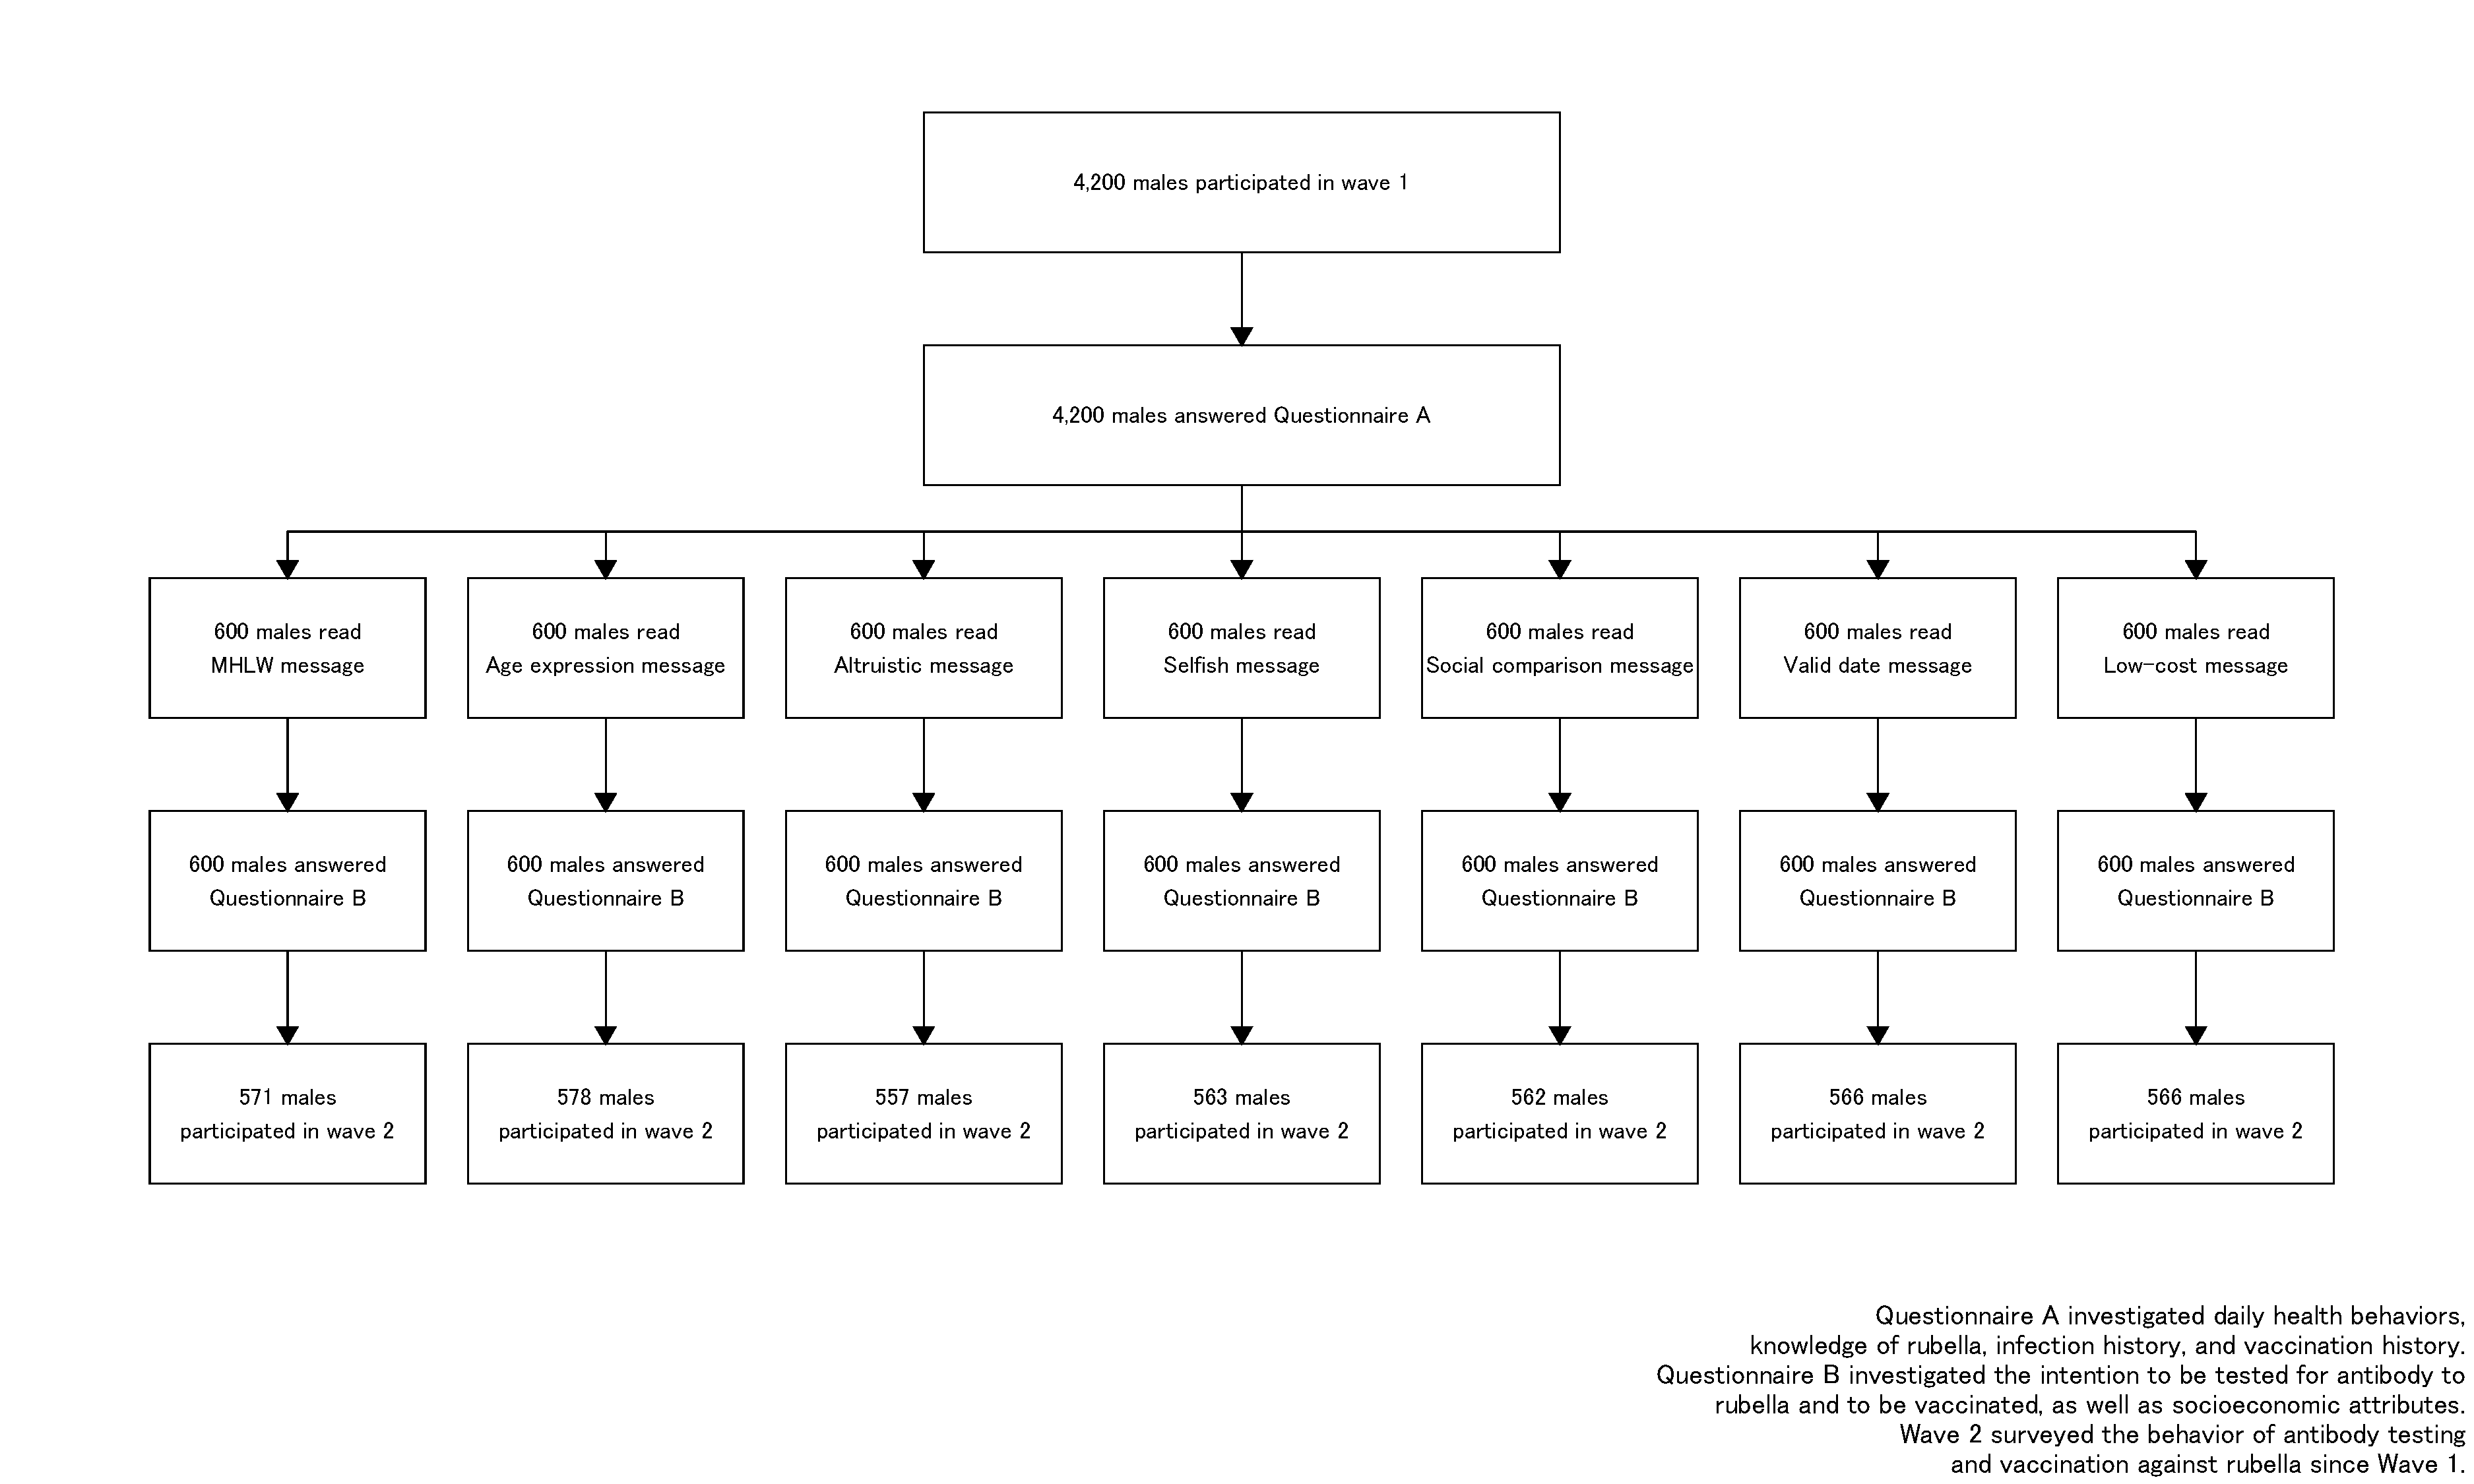
\includegraphics[width=1.5\linewidth,angle=90]{C:/Users/vge00/Desktop/MHLWRubellaNudge/publish/RIETI/webRCT/webRCT_files/figure-latex/flowchart-1} \caption{オンライン調査の概要}\label{fig:flowchart}
\end{figure}

\begin{table}[!h]

\caption{\label{tab:covlist}共変量の一覧}
\centering
\fontsize{9}{11}\selectfont
\begin{tabular}[t]{l>{\raggedright\arraybackslash}p{30em}cc}
\toprule
  & 変数の説明 & Mean & Std.Dev.\\
\midrule
age & (Wave1) 生まれ年と生まれつきに基づいて計算した2019年4月時点の年齢 & 48.66 & 5.69\\
coupon2019 & (Wave1) 2019年4月時点で40歳以上46歳以下(2019年度クーポン券配布対象)ならば1を取るダミー変数 & 0.35 & 0.48\\
married & (Wave1) 婚姻したら1を取るダミー変数 & 0.58 & 0.49\\
education & (Wave1) 教育年数 & 14.75 & 2.31\\
exercise\_w1 & (Wave1) 週に1度以上運動やスポーツをしていたら1を取るダミー変数 & 0.22 & 0.42\\
health\_check & (Wave1) 調査時点から過去1年間で職場や自治体の健康診断を受けたら1を取るダミー変数 & 0.68 & 0.46\\
flushot & (Wave1) 毎年インフルエンザワクチンを接種しているならば1を取るダミー変数 & 0.27 & 0.45\\
prob\_social & (Wave1) 40代・50代が風しんに感染する確率はどれくらいか? & 30.38 & 19.87\\
handicap & (Wave1)妊娠初期の女性が風しんに感染したら、障害を持った子供が産まれる可能性があると回答者が信じているならば、1を取るダミー変数 & 0.63 & 0.48\\
severity & (Wave1) 成人男性が風しんに感染すると、重症化する可能性があると回答者が信じているならば、1を取るダミー変数 & 0.92 & 0.27\\
handwash & (Wave2)「前回の調査から今日までの期間で、こまめに手洗い・うがいをしている」という文章に対する5段階評価(1:全く当てはまらない~5:非常に当てはまる) & 3.91 & 1.04\\
temp\_check & (Wave2)「前回の調査から今日までの期間で、こまめに体温を測定している」という文章に対する5段階評価(1:全く当てはまらない~5:非常に当てはまる) & 2.26 & 1.22\\
avoid\_out & (Wave2)「前回の調査から今日までの期間で、外出を控えている」という文章に対する5段階評価(1:全く当てはまらない~7:非常に当てはまる) & 2.96 & 1.20\\
avoid\_crowd & (Wave2)「前回の調査から今日までの期間で、外出するときは、人ごみの多い場所を避けている」という文章に対する5段階評価(1:全く当てはまらない~8:非常に当てはまる) & 3.38 & 1.10\\
wear\_mask & (Wave2)「前回の調査から今日までの期間で、外出するときや人と会うときは、必ずマスクを着用している」という文章に対する5段階評価(1:全く当てはまらない~9:非常に当てはまる) & 3.14 & 1.38\\
\bottomrule
\end{tabular}
\end{table}

\begin{table}

\caption{\label{tab:BalanceWave1Coupon1}Wave 1セレクションデータの共変量のバランステスト(2019年度クーポン券配布対象)}
\centering
\fontsize{9}{11}\selectfont
\begin{tabular}[t]{lcccccccc}
\toprule
\multicolumn{1}{c}{ } & \multicolumn{7}{c}{Treatments} & \multicolumn{1}{c}{ } \\
\cmidrule(l{3pt}r{3pt}){2-8}
  & 厚労省 & 年齢表現 & 利他強調 & 利己強調 & 社会比較 & 有効期限 & 低コスト & P-value (F-test)\\
\midrule
age & 42.862 & 43.046 & 43.135 & 43.045 & 42.909 & 42.906 & 42.866 & 0.874\\
avoid\_crowd & 3.328 & 3.331 & 3.261 & 3.211 & 3.339 & 3.336 & 3.273 & 0.961\\
avoid\_out & 3.082 & 3.047 & 3.028 & 2.805 & 2.896 & 3.038 & 2.926 & 0.492\\
education & 14.654 & 14.473 & 14.595 & 14.205 & 14.099 & 14.348 & 14.575 & 0.416\\
exercise\_w1 & 0.246 & 0.176 & 0.277 & 0.189 & 0.165 & 0.217 & 0.213 & 0.266\\
flushot & 0.238 & 0.260 & 0.203 & 0.144 & 0.140 & 0.239 & 0.236 & 0.092\\
handicap & 0.638 & 0.550 & 0.595 & 0.568 & 0.537 & 0.543 & 0.520 & 0.518\\
handwash & 3.885 & 3.866 & 3.824 & 3.764 & 3.748 & 3.954 & 3.744 & 0.653\\
health\_check & 0.654 & 0.626 & 0.696 & 0.538 & 0.603 & 0.674 & 0.614 & 0.145\\
married & 0.408 & 0.458 & 0.412 & 0.417 & 0.455 & 0.478 & 0.480 & 0.786\\
prob\_social & 27.231 & 30.000 & 26.689 & 30.758 & 26.529 & 28.333 & 27.795 & 0.470\\
severity & 0.892 & 0.954 & 0.926 & 0.894 & 0.926 & 0.964 & 0.913 & 0.196\\
temp\_check & 2.180 & 2.260 & 2.380 & 2.179 & 2.226 & 2.145 & 2.157 & 0.717\\
wear\_mask & 2.951 & 3.063 & 3.113 & 3.033 & 2.965 & 3.115 & 3.174 & 0.849\\
\bottomrule
\end{tabular}
\end{table}

\begin{table}

\caption{\label{tab:BalanceWave2Coupon1}Wave 2セレクションデータの共変量のバランステスト(2019年度クーポン券配布対象)}
\centering
\fontsize{9}{11}\selectfont
\begin{tabular}[t]{lcccccccc}
\toprule
\multicolumn{1}{c}{ } & \multicolumn{7}{c}{Treatments} & \multicolumn{1}{c}{ } \\
\cmidrule(l{3pt}r{3pt}){2-8}
  & 厚労省 & 年齢表現 & 利他強調 & 利己強調 & 社会比較 & 有効期限 & 低コスト & P-value (F-test)\\
\midrule
age & 42.861 & 43.059 & 43.102 & 43.036 & 42.893 & 42.898 & 42.964 & 0.951\\
avoid\_crowd & 3.296 & 3.336 & 3.273 & 3.234 & 3.350 & 3.305 & 3.324 & 0.991\\
avoid\_out & 3.096 & 3.034 & 3.047 & 2.793 & 2.932 & 3.025 & 2.928 & 0.531\\
education & 14.496 & 14.471 & 14.547 & 14.126 & 14.010 & 14.407 & 14.595 & 0.437\\
exercise\_w1 & 0.252 & 0.185 & 0.266 & 0.171 & 0.165 & 0.195 & 0.225 & 0.355\\
flushot & 0.235 & 0.261 & 0.227 & 0.135 & 0.146 & 0.246 & 0.207 & 0.138\\
handicap & 0.652 & 0.563 & 0.602 & 0.568 & 0.544 & 0.542 & 0.514 & 0.446\\
handwash & 3.861 & 3.916 & 3.797 & 3.757 & 3.767 & 3.915 & 3.829 & 0.853\\
health\_check & 0.643 & 0.639 & 0.680 & 0.532 & 0.631 & 0.661 & 0.640 & 0.359\\
married & 0.391 & 0.454 & 0.391 & 0.360 & 0.437 & 0.466 & 0.477 & 0.474\\
prob\_social & 27.739 & 30.504 & 27.031 & 31.982 & 26.311 & 28.729 & 28.018 & 0.325\\
severity & 0.896 & 0.950 & 0.922 & 0.883 & 0.913 & 0.975 & 0.910 & 0.143\\
temp\_check & 2.139 & 2.235 & 2.414 & 2.126 & 2.204 & 2.203 & 2.117 & 0.519\\
wear\_mask & 2.930 & 3.076 & 3.109 & 3.009 & 3.010 & 3.144 & 3.207 & 0.777\\
\bottomrule
\end{tabular}
\end{table}

\begin{table}

\caption{\label{tab:BalanceWave1Coupon0}Wave 1セレクションデータの共変量のバランステスト(2019年度クーポン券配布対象外)}
\centering
\fontsize{9}{11}\selectfont
\begin{tabular}[t]{lcccccccc}
\toprule
\multicolumn{1}{c}{ } & \multicolumn{7}{c}{Treatments} & \multicolumn{1}{c}{ } \\
\cmidrule(l{3pt}r{3pt}){2-8}
  & 厚労省 & 年齢表現 & 利他強調 & 利己強調 & 社会比較 & 有効期限 & 低コスト & P-value (F-test)\\
\midrule
age & 51.632 & 51.408 & 51.226 & 51.657 & 51.582 & 51.545 & 51.502 & 0.709\\
avoid\_crowd & 3.307 & 3.378 & 3.429 & 3.250 & 3.306 & 3.296 & 3.455 & 0.387\\
avoid\_out & 2.903 & 2.917 & 2.919 & 2.884 & 2.825 & 2.966 & 2.982 & 0.860\\
education & 14.572 & 14.655 & 14.530 & 14.830 & 14.566 & 14.634 & 14.393 & 0.565\\
exercise\_w1 & 0.156 & 0.193 & 0.239 & 0.230 & 0.183 & 0.203 & 0.218 & 0.281\\
flushot & 0.228 & 0.244 & 0.197 & 0.270 & 0.275 & 0.228 & 0.251 & 0.456\\
handicap & 0.596 & 0.630 & 0.607 & 0.617 & 0.574 & 0.626 & 0.619 & 0.878\\
handwash & 3.803 & 3.883 & 3.900 & 3.778 & 3.817 & 3.833 & 3.892 & 0.844\\
health\_check & 0.632 & 0.664 & 0.701 & 0.683 & 0.653 & 0.659 & 0.644 & 0.751\\
married & 0.600 & 0.588 & 0.628 & 0.657 & 0.602 & 0.549 & 0.619 & 0.335\\
prob\_social & 26.920 & 31.387 & 30.983 & 28.522 & 29.442 & 27.846 & 31.925 & 0.033\\
severity & 0.920 & 0.933 & 0.919 & 0.970 & 0.940 & 0.931 & 0.908 & 0.192\\
temp\_check & 2.139 & 2.248 & 2.210 & 2.083 & 2.192 & 2.086 & 2.270 & 0.499\\
wear\_mask & 3.071 & 3.191 & 3.157 & 3.148 & 2.961 & 2.966 & 3.068 & 0.434\\
\bottomrule
\end{tabular}
\end{table}

\begin{table}

\caption{\label{tab:BalanceWave2Coupon0}Wave 1セレクションデータの共変量のバランステスト(2019年度クーポン券配布対象外)}
\centering
\fontsize{9}{11}\selectfont
\begin{tabular}[t]{lcccccccc}
\toprule
\multicolumn{1}{c}{ } & \multicolumn{7}{c}{Treatments} & \multicolumn{1}{c}{ } \\
\cmidrule(l{3pt}r{3pt}){2-8}
  & 厚労省 & 年齢表現 & 利他強調 & 利己強調 & 社会比較 & 有効期限 & 低コスト & P-value (F-test)\\
\midrule
age & 51.695 & 51.394 & 51.179 & 51.662 & 51.421 & 51.605 & 51.512 & 0.576\\
avoid\_crowd & 3.295 & 3.361 & 3.447 & 3.239 & 3.313 & 3.309 & 3.433 & 0.460\\
avoid\_out & 2.886 & 2.889 & 2.932 & 2.866 & 2.855 & 2.964 & 2.941 & 0.960\\
education & 14.505 & 14.620 & 14.553 & 14.876 & 14.593 & 14.610 & 14.345 & 0.428\\
exercise\_w1 & 0.159 & 0.194 & 0.232 & 0.229 & 0.173 & 0.211 & 0.202 & 0.455\\
flushot & 0.223 & 0.245 & 0.189 & 0.264 & 0.280 & 0.215 & 0.241 & 0.389\\
handicap & 0.609 & 0.634 & 0.637 & 0.617 & 0.584 & 0.628 & 0.606 & 0.934\\
handwash & 3.823 & 3.889 & 3.926 & 3.751 & 3.836 & 3.861 & 3.867 & 0.778\\
health\_check & 0.632 & 0.667 & 0.684 & 0.677 & 0.645 & 0.673 & 0.631 & 0.848\\
married & 0.591 & 0.560 & 0.611 & 0.652 & 0.598 & 0.547 & 0.596 & 0.418\\
prob\_social & 27.409 & 31.296 & 30.368 & 29.055 & 30.187 & 28.072 & 32.118 & 0.157\\
severity & 0.923 & 0.935 & 0.926 & 0.970 & 0.935 & 0.933 & 0.921 & 0.484\\
temp\_check & 2.095 & 2.204 & 2.221 & 2.100 & 2.136 & 2.085 & 2.182 & 0.833\\
wear\_mask & 3.082 & 3.176 & 3.116 & 3.144 & 2.977 & 2.942 & 3.010 & 0.522\\
\bottomrule
\end{tabular}
\end{table}

\begin{table}

\caption{\label{tab:AprioriPowerAnalysis}検出力80\%・有意水準5\%を保つために必要な二群の平均の差}
\centering
\fontsize{9}{11}\selectfont
\begin{threeparttable}
\begin{tabular}[t]{lcccccccc}
\toprule
\multicolumn{1}{c}{ } & \multicolumn{4}{c}{Wave 1セレクションデータ} & \multicolumn{4}{c}{Wave 2セレクションデータ} \\
\cmidrule(l{3pt}r{3pt}){2-5} \cmidrule(l{3pt}r{3pt}){6-9}
\multicolumn{1}{c}{ } & \multicolumn{2}{c}{クーポン配布対象} & \multicolumn{2}{c}{クーポン配布対象外} & \multicolumn{2}{c}{クーポン配布対象} & \multicolumn{2}{c}{クーポン配布対象外} \\
\cmidrule(l{3pt}r{3pt}){2-3} \cmidrule(l{3pt}r{3pt}){4-5} \cmidrule(l{3pt}r{3pt}){6-7} \cmidrule(l{3pt}r{3pt}){8-9}
介入群 & N & 二群の差 & N  & 二群の差  & N   & 二群の差   & N    & 二群の差   \\
\midrule
厚労省 & 130 &  & 250 &  & 115 &  & 220 & \\
年齢表現 & 131 & 0.0696 & 238 & 0.0508 & 119 & 0.0736 & 216 & 0.0538\\
利他強調 & 148 & 0.0676 & 234 & 0.0511 & 128 & 0.0723 & 190 & 0.0556\\
利己強調 & 132 & 0.0695 & 230 & 0.0513 & 111 & 0.0749 & 201 & 0.0548\\
社会比較 & 121 & 0.0711 & 251 & 0.0502 & 103 & 0.0764 & 214 & 0.0539\\
有効期限 & 138 & 0.0687 & 246 & 0.0504 & 118 & 0.0737 & 223 & 0.0534\\
低コスト & 127 & 0.0702 & 239 & 0.0508 & 111 & 0.0749 & 203 & 0.0547\\
\bottomrule
\end{tabular}
\begin{tablenotes}
\item 注)効果量から二群の平均の差の絶対値を計算するときに、標準偏差が0.2であることを仮定している。
\end{tablenotes}
\end{threeparttable}
\end{table}

\begin{table}

\caption{\label{tab:RegCoupon1}2019年度クーポン券配布対象者に限定した 抗体検査とワクチン接種の線形確率モデルの推定結果}
\centering
\fontsize{9}{11}\selectfont
\begin{threeparttable}
\begin{tabular}[t]{lcccccccc}
\toprule
\multicolumn{1}{c}{ } & \multicolumn{4}{c}{意向} & \multicolumn{4}{c}{第1回調査以降の行動} \\
\cmidrule(l{3pt}r{3pt}){2-5} \cmidrule(l{3pt}r{3pt}){6-9}
\multicolumn{1}{c}{ } & \multicolumn{2}{c}{抗体検査} & \multicolumn{2}{c}{ワクチン接種} & \multicolumn{2}{c}{抗体検査} & \multicolumn{2}{c}{抗体検査×ワクチン接種} \\
\cmidrule(l{3pt}r{3pt}){2-3} \cmidrule(l{3pt}r{3pt}){4-5} \cmidrule(l{3pt}r{3pt}){6-7} \cmidrule(l{3pt}r{3pt}){8-9}
  & (1) & (2) & (3) & (4) & (5) & (6) & (7) & (8)\\
\midrule
年齢表現 & 0.021 & 0.013 & 0.020 & 0.006 & 0.032 & 0.030 & 0.008 & 0.007\\
 & (0.051) & (0.051) & (0.061) & (0.061) & (0.029) & (0.028) & (0.015) & (0.015)\\
利他強調 & 0.144*** & 0.151*** & 0.024 & 0.022 & 0.075** & 0.073** & 0.038* & 0.037*\\
 & (0.053) & (0.052) & (0.059) & (0.059) & (0.032) & (0.032) & (0.021) & (0.021)\\
利己強調 & 0.073 & 0.091* & 0.039 & 0.048 & 0.055* & 0.067** & 0.018 & 0.022\\
 & (0.053) & (0.052) & (0.061) & (0.061) & (0.032) & (0.032) & (0.018) & (0.018)\\
社会比較 & 0.040 & 0.079 & 0.014 & 0.021 & 0.053 & 0.065** & 0.040* & 0.045*\\
 & (0.053) & (0.052) & (0.062) & (0.061) & (0.033) & (0.033) & (0.023) & (0.023)\\
有効期限 & 0.031 & 0.026 & -0.010 & -0.021 & 0.008 & 0.008 & 0.000 & 0.001\\
 & (0.051) & (0.050) & (0.060) & (0.060) & (0.025) & (0.025) & (0.012) & (0.012)\\
低コスト & 0.052 & 0.053 & 0.018 & 0.014 & 0.037 & 0.041 & 0.018 & 0.022\\
 & (0.053) & (0.051) & (0.062) & (0.061) & (0.030) & (0.029) & (0.018) & (0.018)\\
\midrule
Num.Obs. & 927 & 881 & 927 & 881 & 805 & 805 & 805 & 805\\
R2 & 0.010 & 0.140 & 0.001 & 0.117 & 0.009 & 0.037 & 0.009 & 0.036\\
R2 Adj. & 0.004 & 0.120 & -0.006 & 0.097 & 0.002 & 0.012 & 0.002 & 0.011\\
共変量 &  & X &  & X &  & X &  & X\\
\bottomrule
\end{tabular}
\begin{tablenotes}
\item 注)* p < 0.1、** p < 0.05、*** p < 0.01。頑健標準誤差を使用している。 共変量は補論\ref{addtab}の表\ref{tab:covlist}に示した変数をすべて使用している。
\end{tablenotes}
\end{threeparttable}
\end{table}

\begin{table}

\caption{\label{tab:altbase-reg-coupon1}利他強調メッセージと比較した介入群の効果 (2019年度クーポン券配布対象者)}
\centering
\fontsize{9}{11}\selectfont
\begin{threeparttable}
\begin{tabular}[t]{lcccccccc}
\toprule
\multicolumn{1}{c}{ } & \multicolumn{4}{c}{意向} & \multicolumn{4}{c}{第1回調査以降の行動} \\
\cmidrule(l{3pt}r{3pt}){2-5} \cmidrule(l{3pt}r{3pt}){6-9}
\multicolumn{1}{c}{ } & \multicolumn{2}{c}{抗体検査} & \multicolumn{2}{c}{ワクチン接種} & \multicolumn{2}{c}{抗体検査} & \multicolumn{2}{c}{抗体検査×ワクチン接種} \\
\cmidrule(l{3pt}r{3pt}){2-3} \cmidrule(l{3pt}r{3pt}){4-5} \cmidrule(l{3pt}r{3pt}){6-7} \cmidrule(l{3pt}r{3pt}){8-9}
  & (1) & (2) & (3) & (4) & (5) & (6) & (7) & (8)\\
\midrule
厚労省 & -0.144*** & -0.151*** & -0.024 & -0.022 & -0.075** & -0.073** & -0.038* & -0.037*\\
 & (0.053) & (0.052) & (0.059) & (0.059) & (0.032) & (0.032) & (0.021) & (0.021)\\
年齢表現 & -0.122** & -0.138*** & -0.004 & -0.016 & -0.042 & -0.043 & -0.030 & -0.029\\
 & (0.054) & (0.052) & (0.060) & (0.058) & (0.036) & (0.036) & (0.022) & (0.022)\\
利己強調 & -0.071 & -0.061 & 0.015 & 0.026 & -0.019 & -0.006 & -0.020 & -0.014\\
 & (0.055) & (0.054) & (0.060) & (0.058) & (0.039) & (0.038) & (0.024) & (0.023)\\
社会比較 & -0.103* & -0.072 & -0.009 & -0.001 & -0.022 & -0.008 & 0.002 & 0.008\\
 & (0.056) & (0.054) & (0.061) & (0.058) & (0.039) & (0.039) & (0.028) & (0.028)\\
有効期限 & -0.112** & -0.125** & -0.033 & -0.043 & -0.067** & -0.066** & -0.038* & -0.036*\\
 & (0.053) & (0.052) & (0.058) & (0.058) & (0.033) & (0.033) & (0.021) & (0.021)\\
低コスト & -0.092* & -0.098* & -0.006 & -0.008 & -0.037 & -0.032 & -0.020 & -0.014\\
 & (0.055) & (0.052) & (0.060) & (0.058) & (0.037) & (0.036) & (0.024) & (0.024)\\
\midrule
Num.Obs. & 927 & 881 & 927 & 881 & 805 & 805 & 805 & 805\\
R2 & 0.010 & 0.140 & 0.001 & 0.117 & 0.009 & 0.037 & 0.009 & 0.036\\
R2 Adj. & 0.004 & 0.120 & -0.006 & 0.097 & 0.002 & 0.012 & 0.002 & 0.011\\
共変量 &  & X &  & X &  & X &  & X\\
\bottomrule
\end{tabular}
\begin{tablenotes}
\item 注)* p < 0.1、** p < 0.05、*** p < 0.01。頑健標準誤差を使用している。 共変量は補論\ref{addtab}の表\ref{tab:covlist}に示した変数をすべて使用している。
\end{tablenotes}
\end{threeparttable}
\end{table}

\begin{table}

\caption{\label{tab:RegCoupon0}2019年度クーポン券配布対象外の男性に限定した 抗体検査とワクチン接種の線形確率モデルの推定結果}
\centering
\fontsize{9}{11}\selectfont
\begin{threeparttable}
\begin{tabular}[t]{lcccccccc}
\toprule
\multicolumn{1}{c}{ } & \multicolumn{4}{c}{意向} & \multicolumn{4}{c}{第1回調査以降の行動} \\
\cmidrule(l{3pt}r{3pt}){2-5} \cmidrule(l{3pt}r{3pt}){6-9}
\multicolumn{1}{c}{ } & \multicolumn{2}{c}{抗体検査} & \multicolumn{2}{c}{ワクチン接種} & \multicolumn{2}{c}{抗体検査} & \multicolumn{2}{c}{抗体検査×ワクチン接種} \\
\cmidrule(l{3pt}r{3pt}){2-3} \cmidrule(l{3pt}r{3pt}){4-5} \cmidrule(l{3pt}r{3pt}){6-7} \cmidrule(l{3pt}r{3pt}){8-9}
  & (1) & (2) & (3) & (4) & (5) & (6) & (7) & (8)\\
\midrule
年齢表現 & -0.024 & -0.036 & -0.066 & -0.101** & 0.005 & 0.004 & 0.005 & 0.005\\
 & (0.040) & (0.038) & (0.045) & (0.043) & (0.008) & (0.008) & (0.005) & (0.005)\\
利他強調 & 0.053 & 0.053 & -0.028 & -0.059 & 0.017 & 0.016 & 0.005 & 0.005\\
 & (0.042) & (0.042) & (0.045) & (0.045) & (0.011) & (0.011) & (0.005) & (0.005)\\
利己強調 & 0.041 & 0.026 & -0.028 & -0.053 & 0.010 & 0.009 & 0.005 & 0.005\\
 & (0.042) & (0.040) & (0.046) & (0.043) & (0.010) & (0.010) & (0.005) & (0.005)\\
社会比較 & -0.037 & -0.043 & -0.082* & -0.098** & 0.023* & 0.022* & 0.000 & 0.000\\
 & (0.039) & (0.038) & (0.045) & (0.042) & (0.012) & (0.012) &  & (0.001)\\
有効期限 & 0.029 & 0.029 & -0.028 & -0.043 & 0.009 & 0.009 & 0.004 & 0.005\\
 & (0.041) & (0.039) & (0.045) & (0.042) & (0.009) & (0.009) & (0.004) & (0.005)\\
低コスト & 0.063 & 0.034 & -0.030 & -0.052 & 0.005 & 0.006 & 0.000 & 0.000\\
 & (0.042) & (0.040) & (0.045) & (0.043) & (0.008) & (0.008) &  & (0.001)\\
\midrule
Num.Obs. & 1688 & 1578 & 1688 & 1578 & 1467 & 1467 & 1467 & 1467\\
R2 & 0.006 & 0.107 & 0.003 & 0.125 & 0.004 & 0.019 & 0.002 & 0.013\\
R2 Adj. & 0.003 & 0.095 & -0.001 & 0.113 & 0.000 & 0.005 & -0.002 & -0.001\\
共変量 &  & X &  & X &  & X &  & X\\
\bottomrule
\end{tabular}
\begin{tablenotes}
\item 注)* p < 0.1、** p < 0.05、*** p < 0.01。頑健標準誤差を使用している。 共変量は補論\ref{addtab}の表\ref{tab:covlist}に示した変数をすべて使用している。 社会比較メッセージ群と低コストダミー群の回答者は全員ワクチン接種をしていないので、 列(7)の社会比較ダミーと低コストダミーの標準誤差は計算できない。
\end{tablenotes}
\end{threeparttable}
\end{table}

\clearpage

\hypertarget{ux30b5ux30f3ux30d7ux30ebux30bbux30ecux30afux30b7ux30e7ux30f3ux3068ux30a2ux30a6ux30c8ux30abux30e0ux5909ux6570ux306eux5b9aux7fa9ux3092ux5909ux66f4ux3057ux305fux5206ux6790}{%
\section{サンプルセレクションとアウトカム変数の定義を変更した分析}\label{ux30b5ux30f3ux30d7ux30ebux30bbux30ecux30afux30b7ux30e7ux30f3ux3068ux30a2ux30a6ux30c8ux30abux30e0ux5909ux6570ux306eux5b9aux7fa9ux3092ux5909ux66f4ux3057ux305fux5206ux6790}}

\begin{table}

\caption{\label{tab:c1balancetestw2coupon1}新しいサンプルセレクション定義に従ったWave 2データのバランステストの結果(2019年度クーポン券配布対象)}
\centering
\fontsize{9}{11}\selectfont
\begin{tabular}[t]{lcccccccc}
\toprule
\multicolumn{1}{c}{ } & \multicolumn{7}{c}{Treatments} & \multicolumn{1}{c}{ } \\
\cmidrule(l{3pt}r{3pt}){2-8}
  & 厚労省 & 年齢表現 & 利他強調 & 利己強調 & 社会比較 & 有効期限 & 低コスト & P-value (F-test)\\
\midrule
age & 42.869 & 43.063 & 43.099 & 43.016 & 42.948 & 42.901 & 42.893 & 0.949\\
avoid\_crowd & 3.328 & 3.331 & 3.261 & 3.211 & 3.339 & 3.336 & 3.273 & 0.961\\
avoid\_out & 3.082 & 3.047 & 3.028 & 2.805 & 2.896 & 3.038 & 2.926 & 0.492\\
education & 14.598 & 14.457 & 14.592 & 14.236 & 14.130 & 14.267 & 14.603 & 0.519\\
exercise\_w1 & 0.262 & 0.181 & 0.289 & 0.179 & 0.165 & 0.198 & 0.215 & 0.128\\
flushot & 0.238 & 0.268 & 0.211 & 0.130 & 0.148 & 0.244 & 0.215 & 0.073\\
handicap & 0.648 & 0.551 & 0.599 & 0.553 & 0.539 & 0.527 & 0.496 & 0.276\\
handwash & 3.885 & 3.866 & 3.824 & 3.764 & 3.748 & 3.954 & 3.744 & 0.653\\
health\_check & 0.656 & 0.638 & 0.683 & 0.528 & 0.617 & 0.664 & 0.620 & 0.215\\
married & 0.402 & 0.465 & 0.408 & 0.415 & 0.452 & 0.473 & 0.479 & 0.767\\
prob\_social & 27.623 & 30.079 & 26.901 & 30.976 & 26.870 & 28.015 & 27.851 & 0.550\\
severity & 0.902 & 0.953 & 0.930 & 0.886 & 0.922 & 0.977 & 0.909 & 0.094\\
temp\_check & 2.180 & 2.260 & 2.380 & 2.179 & 2.226 & 2.145 & 2.157 & 0.717\\
wear\_mask & 2.951 & 3.063 & 3.113 & 3.033 & 2.965 & 3.115 & 3.174 & 0.849\\
\bottomrule
\end{tabular}
\end{table}

\begin{table}

\caption{\label{tab:c1balancetestw2coupon0}新しいサンプルセレクション定義に従ったWave 2データのバランステストの結果(2019年度クーポン券配布対象外)}
\centering
\fontsize{9}{11}\selectfont
\begin{tabular}[t]{lcccccccc}
\toprule
\multicolumn{1}{c}{ } & \multicolumn{7}{c}{Treatments} & \multicolumn{1}{c}{ } \\
\cmidrule(l{3pt}r{3pt}){2-8}
  & 厚労省 & 年齢表現 & 利他強調 & 利己強調 & 社会比較 & 有効期限 & 低コスト & P-value (F-test)\\
\midrule
age & 42.869 & 43.063 & 43.099 & 43.016 & 42.948 & 42.901 & 42.893 & 0.949\\
avoid\_crowd & 3.328 & 3.331 & 3.261 & 3.211 & 3.339 & 3.336 & 3.273 & 0.961\\
avoid\_out & 3.082 & 3.047 & 3.028 & 2.805 & 2.896 & 3.038 & 2.926 & 0.492\\
education & 14.598 & 14.457 & 14.592 & 14.236 & 14.130 & 14.267 & 14.603 & 0.519\\
exercise\_w1 & 0.262 & 0.181 & 0.289 & 0.179 & 0.165 & 0.198 & 0.215 & 0.128\\
flushot & 0.238 & 0.268 & 0.211 & 0.130 & 0.148 & 0.244 & 0.215 & 0.073\\
handicap & 0.648 & 0.551 & 0.599 & 0.553 & 0.539 & 0.527 & 0.496 & 0.276\\
handwash & 3.885 & 3.866 & 3.824 & 3.764 & 3.748 & 3.954 & 3.744 & 0.653\\
health\_check & 0.656 & 0.638 & 0.683 & 0.528 & 0.617 & 0.664 & 0.620 & 0.215\\
married & 0.402 & 0.465 & 0.408 & 0.415 & 0.452 & 0.473 & 0.479 & 0.767\\
prob\_social & 27.623 & 30.079 & 26.901 & 30.976 & 26.870 & 28.015 & 27.851 & 0.550\\
severity & 0.902 & 0.953 & 0.930 & 0.886 & 0.922 & 0.977 & 0.909 & 0.094\\
temp\_check & 2.180 & 2.260 & 2.380 & 2.179 & 2.226 & 2.145 & 2.157 & 0.717\\
wear\_mask & 2.951 & 3.063 & 3.113 & 3.033 & 2.965 & 3.115 & 3.174 & 0.849\\
\bottomrule
\end{tabular}
\end{table}

ここでは、第2回調査の抗体検査の受検行動やワクチン接種行動の回答に
想起バイアスが伴うことを考慮した分析を行う。
第2回調査はそれぞれの行動を第1回調査以前に行ったかどうかを調査している。
この時期の回答に想起バイアスが伴うならば、
本論の分析のように第2回調査で第1回調査以前に行動したと回答した人を除くべきではない。
そこで、我々は第2回調査の行動の回答に想起バイアスが伴うことを仮定して、
第1回調査の調査ですでに抗体検査もしくはワクチン接種を受けた男性だけを除いて、
ナッジ・メッセージの行動に対する効果を推定する。
なお、第2回調査で第1回調査以前に抗体検査もしくはワクチン接種を受けたと回答した人はサンプルに含まれている。

本論と同様に、
我々は2019年度にクーポン券を自動的に受け取っているかどうかでサンプルを分割して、
サブサンプルを用いてナッジ・メッセージの効果を推定する。
表\ref{tab:c1balancetestw2coupon1}と表\ref{tab:c1balancetestw2coupon0}は共変量のバランステストの結果であり、
回答者の観察可能な特徴は群間でシステマティックに異ならないことを示している。

また、アウトカム変数の定義も本論のものから変更する。
本論では、第1回調査以降に抗体検査を受検したら1を取るアウトカム変数と
第1回調査以降に抗体検査を受検し、ワクチンによって抗体を新たに獲得したら1を取るダミー変数でを用いた。
対して、この補論では、
第2回調査で時期に関わらず抗体検査を受検したと回答したら1を取るダミー変数と
第2回調査で時期に関わらず抗体検査を受検し、
時期に関わらずワクチンによって抗体を獲得したら1を取るダミー変数である。

\hypertarget{ux5e74ux5ea6ux30afux30fcux30ddux30f3ux5238ux914dux5e03ux5bfeux8c61ux8005ux306bux9650ux5b9aux3057ux305fux5206ux6790}{%
\subsection{2019年度クーポン券配布対象者に限定した分析}\label{ux5e74ux5ea6ux30afux30fcux30ddux30f3ux5238ux914dux5e03ux5bfeux8c61ux8005ux306bux9650ux5b9aux3057ux305fux5206ux6790}}

始めに、2019年度ににクーポン券が送付された40歳以上46歳以下の男性グループにおける、
ナッジ・メッセージの行動に対する効果を推定する。

\begin{figure}[t]
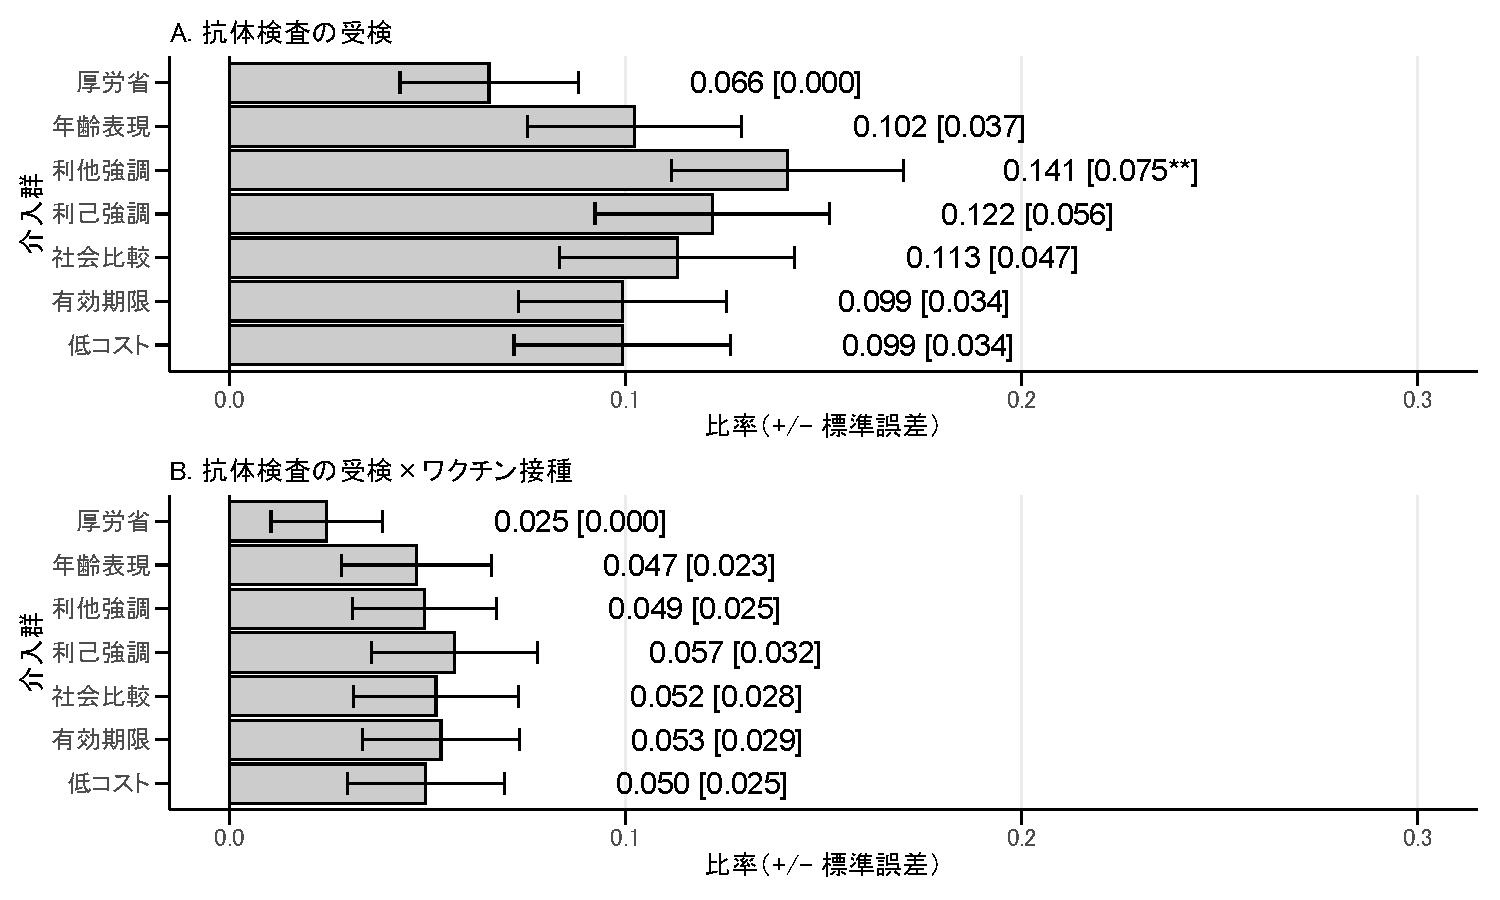
\includegraphics{C:/Users/vge00/Desktop/MHLWRubellaNudge/publish/RIETI/webRCT/webRCT_files/figure-latex/c1BehaviorCoupon1-1} \caption{2019年度クーポン券配布対象者に限定した行動に対するナッジ・メッセージの効果。注)図中の数値は各群の比率を示し、角括弧内の数値はナッジ・メッセージの効果の規模(厚労省メッセージ群との差)を示している。効果の統計的な有意性は次の規則に従う:* p < 0.1、** p < 0.05、*** p < 0.01。}\label{fig:c1BehaviorCoupon1}
\end{figure}

図\ref{fig:c1BehaviorCoupon1}は各介入群のWave 2で抗体検査を受検したと回答した比率と
Wave 2で抗体検査とワクチン接種を両方受けたと回答した比率を示している。
結果として、利他強調メッセージは厚労省メッセージよりも抗体検査の受検比率を高めているが、
抗体検査とワクチン接種の両方を促進していない。
厚労省メッセージを読んだ人の約6.6\%は抗体検査を受検したと回答している。
その一方で、利他強調メッセージを読んだ人の約14.1\%は抗体検査を受検したと回答している。
したがって、利他強調メッセージはコントロールよりも7.5\%ポイント抗体検査の受検率を引き上げており、
これはt検定より統計的に5\%水準で有意である。
また、厚労省メッセージを読んだ人の約2.5\%は抗体検査とワクチン接種の両方を受けたと回答している。
その一方で、利他強調メッセージを読んだ人の約4.9\%が
抗体検査とワクチン接種の両方を受けたと回答している。
したがって、利他強調メッセージはコントロールよりもワクチン接種率を2.4\%ポイント高めているが、
これはt検定より統計的に有意でない。

\begin{table}

\caption{\label{tab:c1RegCoupon1}2019年度クーポン券配布対象者に限定した 抗体検査とワクチン接種の線形確率モデルの推定結果}
\centering
\fontsize{9}{11}\selectfont
\begin{threeparttable}
\begin{tabular}[t]{lcccc}
\toprule
\multicolumn{1}{c}{ } & \multicolumn{2}{c}{抗体検査} & \multicolumn{2}{c}{抗体検査×ワクチン接種} \\
\cmidrule(l{3pt}r{3pt}){2-3} \cmidrule(l{3pt}r{3pt}){4-5}
  & (1) & (2) & (3) & (4)\\
\midrule
年齢表現 & 0.037 & 0.033 & 0.023 & 0.022\\
 & (0.035) & (0.035) & (0.024) & (0.023)\\
利他強調 & 0.075** & 0.075** & 0.025 & 0.025\\
 & (0.037) & (0.037) & (0.023) & (0.024)\\
利己強調 & 0.056 & 0.070* & 0.032 & 0.040\\
 & (0.037) & (0.037) & (0.025) & (0.025)\\
社会比較 & 0.047 & 0.058 & 0.028 & 0.033\\
 & (0.037) & (0.037) & (0.025) & (0.026)\\
有効期限 & 0.034 & 0.032 & 0.029 & 0.029\\
 & (0.035) & (0.034) & (0.024) & (0.024)\\
低コスト & 0.034 & 0.035 & 0.025 & 0.028\\
 & (0.035) & (0.035) & (0.024) & (0.024)\\
\midrule
Num.Obs. & 881 & 881 & 881 & 881\\
R2 & 0.005 & 0.029 & 0.002 & 0.031\\
R2 Adj. & -0.002 & 0.007 & -0.005 & 0.008\\
共変量 &  & X &  & X\\
\bottomrule
\end{tabular}
\begin{tablenotes}
\item 注)* p < 0.1、** p < 0.05、*** p < 0.01。頑健標準誤差を使用している。 共変量は補論\ref{addtab}の表\ref{tab:covlist}に示した変数をすべて使用している。
\end{tablenotes}
\end{threeparttable}
\end{table}

利他強調メッセージの効果は
補論\ref{addtab}の表\ref{tab:covlist}で示した個人の観察可能な特徴をコントロールしても変化しない。
表\ref{tab:c1RegCoupon1}はナッジ・メッセージの線形確率モデルの推定結果である。
奇数列はナッジ・メッセージのダミー変数のみを説明変数に加えているので、
これらの結果は二群間のt検定の結果(図\ref{fig:c1BehaviorCoupon1})に対応している。
偶数列はナッジ・メッセージのダミー変数に加えて、個人の観察可能な特徴を説明変数に加えている。
共変量をコントロールすると、利他強調メッセージに加えて、
利己強調メッセージが厚労省メッセージより抗体検査の受検を促進していることが明らかになった。
これは統計的に10\%水準で有意である。

\begin{table}

\caption{\label{tab:c1CtabTesterCoupon1}抗体検査受検者の動き}
\centering
\resizebox{\linewidth}{!}{
\fontsize{9}{11}\selectfont
\begin{threeparttable}
\begin{tabular}[t]{lccccccc}
\toprule
\multicolumn{2}{c}{ } & \multicolumn{2}{c}{抗体検査の受検} & \multicolumn{2}{c}{抗体検査の結果が陰性} & \multicolumn{2}{c}{陰性かつワクチンを接種} \\
\cmidrule(l{3pt}r{3pt}){3-4} \cmidrule(l{3pt}r{3pt}){5-6} \cmidrule(l{3pt}r{3pt}){7-8}
ナッジ・メッセージ & サンプルサイズ & 人数 & 二群比較のp値 & 人数  & 二群比較のp値 & 人数   & 二群比較のp値\\
\midrule
厚労省 & 122 & 8 & - & 3 & - & 3 & -\\
年齢表現 & 127 & 13 & 0.364 & 6 & 1.000 & 6 & 1.000\\
利他強調 & 142 & 20 & 0.070 & 8 & 1.000 & 7 & 1.000\\
利己強調 & 123 & 15 & 0.188 & 7 & 1.000 & 7 & 1.000\\
社会比較 & 115 & 13 & 0.254 & 7 & 0.659 & 6 & 1.000\\
有効期限 & 131 & 13 & 0.369 & 7 & 0.659 & 7 & 1.000\\
低コスト & 121 & 12 & 0.362 & 8 & 0.362 & 6 & 1.000\\
\bottomrule
\end{tabular}
\begin{tablenotes}
\item 注)二群比較は、厚労省メッセージ群とあるナッジ・メッセージの二群をFisherの正確検定で分析している。抗体検査の受検をアウトカムとするとき、抗体検査の受検者数に群間で差がないという帰無仮説を検定している。抗体検査の陰性者をアウトカムとするとき、抗体検査の受検者の中で陰性者の比率に群間で差がないという帰無仮説を検定している。陰性者のワクチン接種をアウトカムとするとき、陰性者の中でワクチン接種の比率に群間で差がないという帰無仮説を検定している。
\end{tablenotes}
\end{threeparttable}}
\end{table}

本論と同様に、
介入に関わらず抗体検査の結果が陰性である人のほとんどがワクチンを接種している。
全体の陰性者のワクチン接種比率は
91.3\%
である(この95\%ブートストラップ信頼区間は
{[}82.6\%, 97.8\%{]}
)。
また、ベイズ定理を用いた間接的な推定より、
陰性者の抗体検査受検率は約26\%で、全体の抗体検査受検率10\%より高い。
陰性者の抗体検査受検率と全体の抗体検査受検率の差の95\%ブートストラップ信頼区間は
{[}0.094, 0.217{]}
である。
これらの結果は、抗体を保有していない人が抗体検査を受検している傾向にあることを示唆しており、
本論の結果と一致する。

\begin{figure}[t]
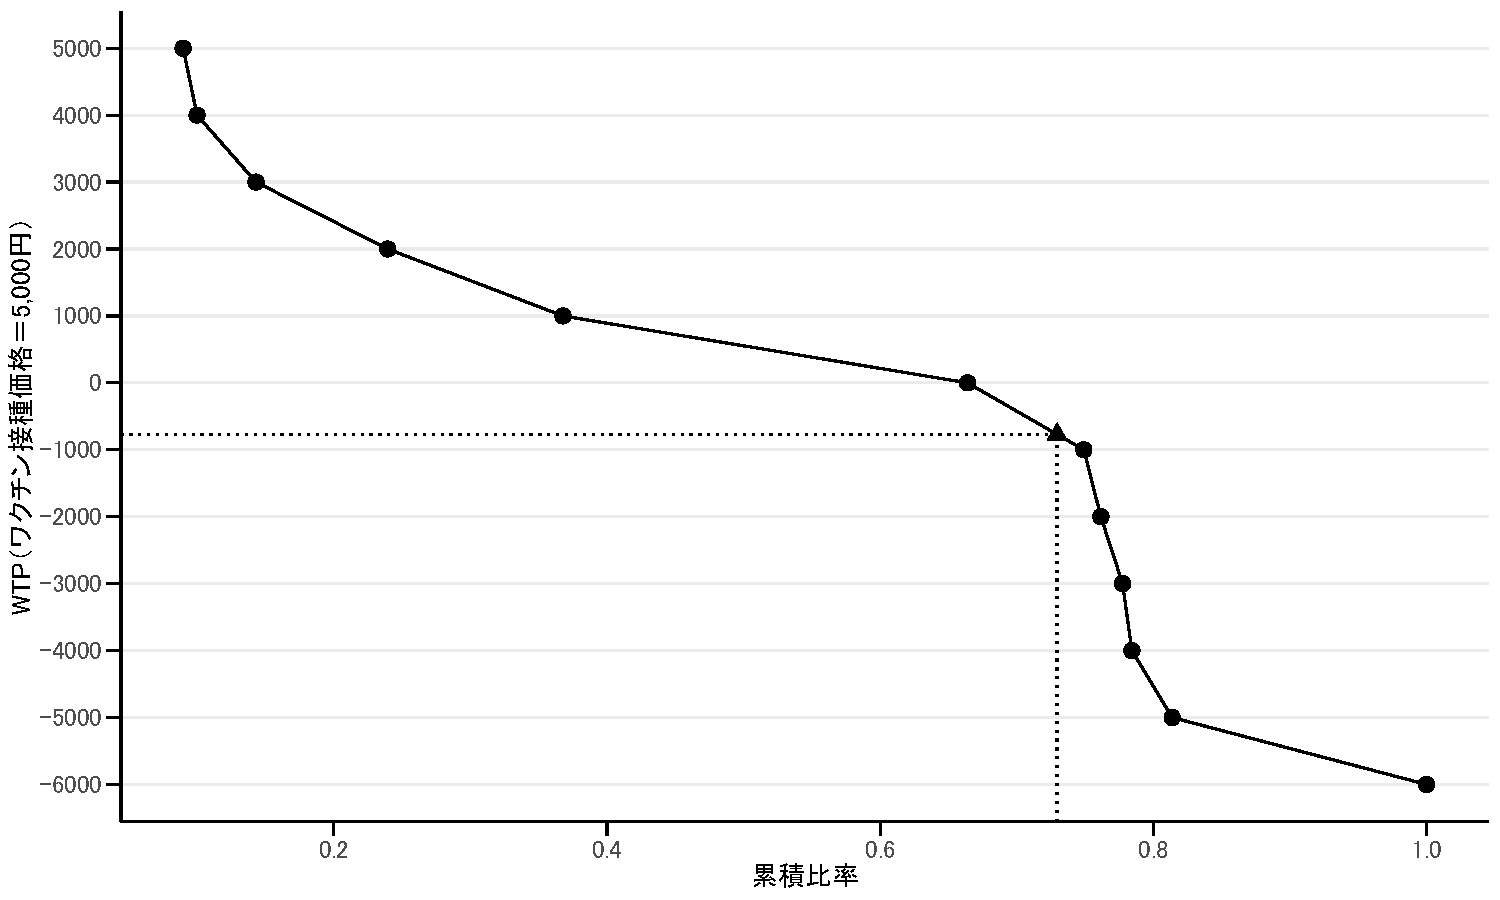
\includegraphics{C:/Users/vge00/Desktop/MHLWRubellaNudge/publish/RIETI/webRCT/webRCT_files/figure-latex/c1demandVaccine-1} \caption{2019年度クーポン券配布対象者の風しんワクチンの需要曲線。データソース:Wave 2データ。注)黒の三角はワクチン接種費用が無料であるときの接種割合と厚労省メッセージの抗体検査受検率を合計した割合と、それに対応するWTPを示している。}\label{fig:c1demandVaccine}
\end{figure}

2019年度にクーポン券を自動的に受け取る人へのナッジ・メッセージの効果を
金銭的な価値で評価することを試みる。
本論で示した方法を用いて、図\ref{fig:c1demandVaccine}に
2019年度に自動的にクーポン券を受け取る人に限定した、風しんワクチン接種の需要曲線を示した。
ワクチン接種が0円で供給されているとき、均衡接種割合は0.664である。

\begin{table}

\caption{\label{tab:c1econvalue}ナッジ・メッセージの金銭的価値の推定}
\centering
\resizebox{\linewidth}{!}{
\fontsize{9}{11}\selectfont
\begin{threeparttable}
\begin{tabular}[t]{lcccccc}
\toprule
\multicolumn{3}{c}{ } & \multicolumn{2}{c}{金銭的価値(日本円)} & \multicolumn{2}{c}{金銭的価値(米ドル)} \\
\cmidrule(l{3pt}r{3pt}){4-5} \cmidrule(l{3pt}r{3pt}){6-7}
ナッジ・メッセージ & 効果の規模 & ベースライン+効果の規模 & 一人当たり & 総額 & 一人当たり  & 総額 \\
\midrule
年齢表現 & 0.037 & 0.766 & 1528.377 & 8.085 & 13.894 & 73.501\\
利他強調 & 0.075 & 0.805 & 3925.285 & 20.765 & 35.684 & 188.771\\
利己強調 & 0.056 & 0.786 & 3285.074 & 17.378 & 29.864 & 157.982\\
社会比較 & 0.047 & 0.777 & 2200.534 & 11.641 & 20.005 & 105.826\\
有効期限 & 0.034 & 0.763 & 1331.690 & 7.045 & 12.106 & 64.042\\
低コスト & 0.034 & 0.763 & 1327.720 & 7.024 & 12.070 & 63.851\\
\bottomrule
\end{tabular}
\begin{tablenotes}
\item 注) 抗体検査の受検に対するナッジ・メッセージの効果を効果の規模として用いた。 ベースラインはワクチン接種費用が無料であるときの接種割合と 厚労省メッセージの抗体検査受検率を合計した割合である。 金銭的価値は一人当たりの価値と それに2020年1月時点でワクチンクーポン券を利用していない人数(529万人)をかけた 総額を示している。 また、金銭的価値は日本円と米ドルで示した(1ドル=110円)。 一人当たりの金銭的価値の単位はそれぞれ1円と1ドルである。 総額で示した金銭的価値の単位はそれぞれ10億円と100万ドルである。
\end{tablenotes}
\end{threeparttable}}
\end{table}

抗体検査の受検確率をナッジ・メッセージの効果量として用いて、
表\ref{tab:c1econvalue}にメッセージの金銭的価値を示した。
第2列は図\ref{fig:c1BehaviorCoupon1}のパネルBで示した比率を示している。
第3列はベースラインの均衡接種割合からメッセージの効果分だけ増やしたときの接種割合を示している。
第4列はそのその接種割合と対応する自治体の追加的な補助金額であり、
これがメッセージの一人当たりの金銭的価値である。
アメリカドルに換算した価値は第6列に示した。
利他強調メッセージの一人当たりの金銭的価値は約3900円(約35ドル)である。
第5列はメッセージの一人当たりの金銭的価値を
2019年度にクーポン券が発行されたにもかかわらず、
1月時点で抗体検査のクーポン券を利用していない人口で掛けた
メッセージの金銭的価値の総額を示している。
アメリカドルに換算した価値は第7列に示している。
利他強調メッセージの金銭的価値の総額はそれぞれ200億円である。

\hypertarget{ux5e74ux5ea6ux30afux30fcux30ddux30f3ux5238ux914dux5e03ux5bfeux8c61ux5916ux306eux7537ux6027ux306bux9650ux5b9aux3057ux305fux5206ux6790}{%
\subsection{2019年度クーポン券配布対象外の男性に限定した分析}\label{ux5e74ux5ea6ux30afux30fcux30ddux30f3ux5238ux914dux5e03ux5bfeux8c61ux5916ux306eux7537ux6027ux306bux9650ux5b9aux3057ux305fux5206ux6790}}

次に、2019年度には、クーポン券の送付対象ではないが、オンデマンドでクーポン券を受け取れる人に限定して、
ナッジ・メッセージの効果を推定する。

\begin{figure}[t]
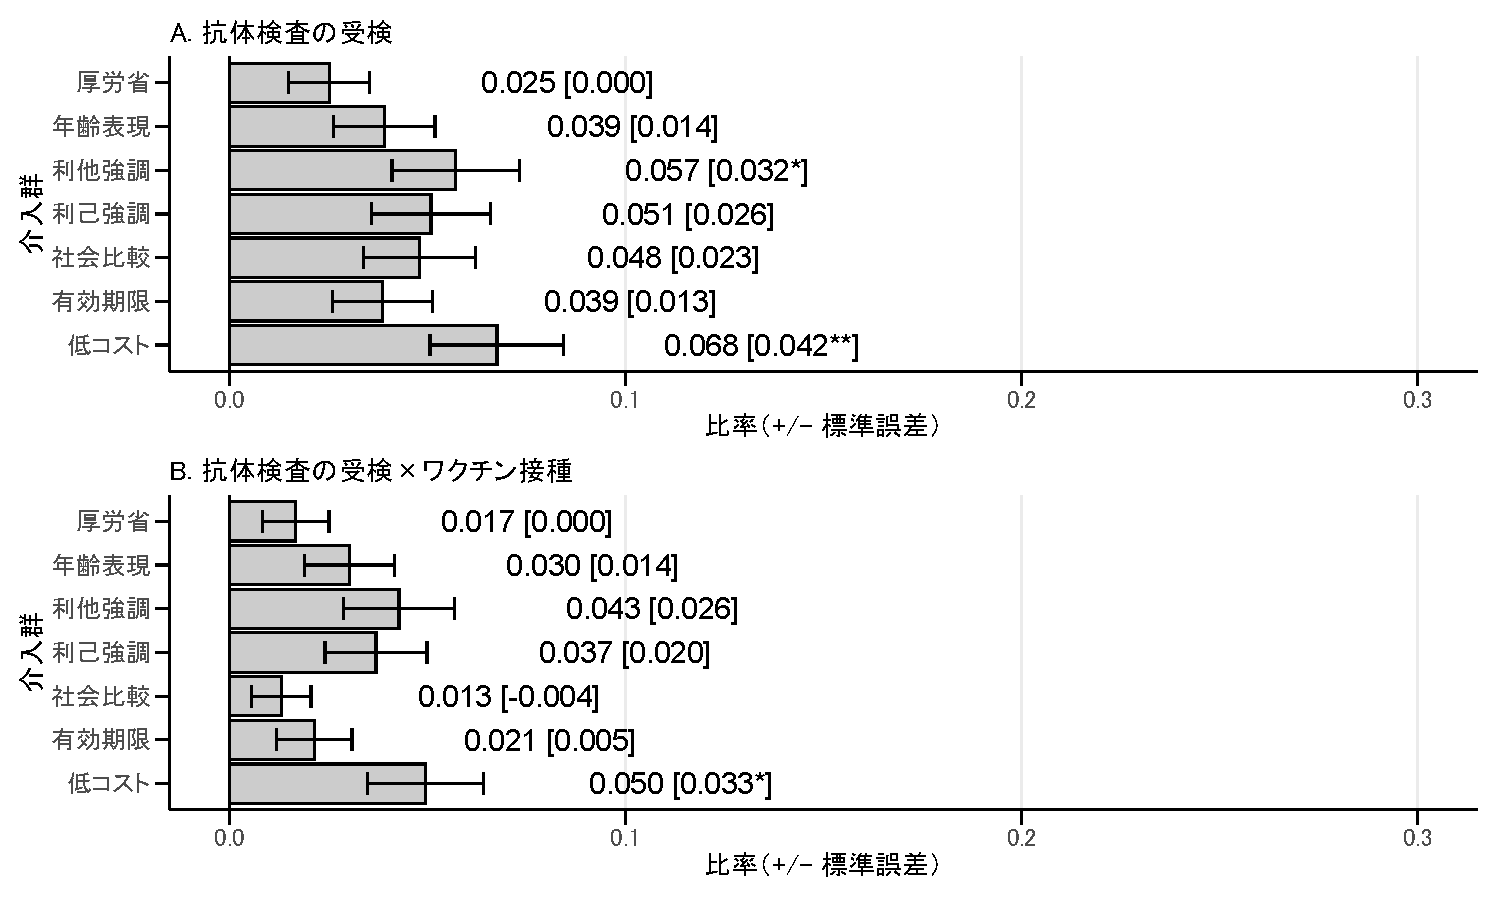
\includegraphics{C:/Users/vge00/Desktop/MHLWRubellaNudge/publish/RIETI/webRCT/webRCT_files/figure-latex/c1BehaviorCoupon0-1} \caption{2019年度クーポン券配布対象外の男性に限定した行動に対するナッジ・メッセージの効果。注)図中の数値は各群の比率を示し、括弧内の数値はナッジ・メッセージの効果の規模を示している。効果の統計的な有意性は次の規則に従う:* p < 0.1、** p < 0.05、*** p < 0.01。}\label{fig:c1BehaviorCoupon0}
\end{figure}

図\ref{fig:c1BehaviorCoupon0}は各介入群のWave 2で抗体検査を受検したと回答した比率と
Wave 2で抗体検査とワクチン接種を両方受けたと回答した比率を示している。
利他強調メッセージと低コストメッセージはコントロールメッセージよりも抗体検査の受検比率を高めていて、
低コストメッセージのみが抗体検査とワクチン接種の両方を受けた比率を高めている。
コントロールメッセージを読んだ人の約2.5\%が抗体検査を受検したと回答し、
約1.7\%が抗体検査とワクチン接種の両方を受けたと回答している。
一方で、利他強調メッセージを読んだ人の約5.7\%が抗体検査を受検したと回答し、
約4.3\%が抗体検査とワクチン接種の両方を受けたと回答している。
よって、利他強調メッセージはコントロールよりも約3.2\%ポイント抗体検査の受検率を高めており、
これは統計的に10\%水準で有意である。
また、利他強調メッセージはコントロールよりもワクチン接種率を約2.6\%ポイント高めているが、
これは統計的に非有意である。
さらに、低コストメッセージ読んだ人の約6.8\%が抗体検査を受検したと回答し、
約5.0\%が抗体検査とワクチン接種の両方を受けたと回答している。
よって、低コストメッセージはコントロールよりも約4.3\%ポイント抗体検査の受検率を引き上げており、
これは統計的に5\%水準で有意である。
また、低コストメッセージはコントロールよりもワクチン接種率を約3.3\%ポイント高めていて、
これは統計的に10\%水準で有意である。

\begin{table}

\caption{\label{tab:c1RegCoupon0}2019年度クーポン券配布対象外の男性に限定した 抗体検査とワクチン接種の線形確率モデルの推定結果}
\centering
\fontsize{9}{11}\selectfont
\begin{threeparttable}
\begin{tabular}[t]{lcccc}
\toprule
\multicolumn{1}{c}{ } & \multicolumn{2}{c}{抗体検査} & \multicolumn{2}{c}{抗体検査×ワクチン接種} \\
\cmidrule(l{3pt}r{3pt}){2-3} \cmidrule(l{3pt}r{3pt}){4-5}
  & (1) & (2) & (3) & (4)\\
\midrule
年齢表現 & 0.014 & 0.015 & 0.014 & 0.015\\
 & (0.016) & (0.017) & (0.014) & (0.014)\\
利他強調 & 0.032* & 0.032* & 0.026 & 0.026\\
 & (0.019) & (0.019) & (0.016) & (0.016)\\
利己強調 & 0.026 & 0.027 & 0.020 & 0.023\\
 & (0.018) & (0.018) & (0.015) & (0.015)\\
社会比較 & 0.023 & 0.023 & -0.004 & -0.003\\
 & (0.017) & (0.018) & (0.011) & (0.011)\\
有効期限 & 0.013 & 0.015 & 0.005 & 0.007\\
 & (0.016) & (0.017) & (0.013) & (0.013)\\
低コスト & 0.042** & 0.042** & 0.033* & 0.032*\\
 & (0.020) & (0.020) & (0.017) & (0.017)\\
\midrule
Num.Obs. & 1578 & 1578 & 1578 & 1578\\
R2 & 0.004 & 0.018 & 0.006 & 0.025\\
R2 Adj. & 0.000 & 0.005 & 0.002 & 0.012\\
共変量 &  & X &  & X\\
\bottomrule
\end{tabular}
\begin{tablenotes}
\item 注)* p < 0.1、** p < 0.05、*** p < 0.01。頑健標準誤差を使用している。 共変量は補論\ref{addtab}の表\ref{tab:covlist}に示した変数をすべて使用している。
\end{tablenotes}
\end{threeparttable}
\end{table}

これらの結果は個人の観察可能な特徴をコントロールしても変化しない。
表\ref{tab:c1RegCoupon0}はナッジ・メッセージの線形確率モデルの推定結果である。
奇数列はナッジ・メッセージのダミー変数のみを説明変数に加えているので、
これらの結果は二群間のt検定の結果(図\ref{fig:c1BehaviorCoupon0})に対応している。
偶数列はナッジ・メッセージのダミー変数に加えて、共変量を説明変数に加えている。
第(2)列は、共変量をコントロールすると、
抗体検査受検に対する利他強調メッセージの効果量は変化していないが、統計的に非有意となる。
また、第(1)列と比較して、標準誤差も大きく変化していない。
よって、利他強調メッセージの統計的な有意性はかなり低い。

\begin{table}

\caption{\label{tab:c1CtabTesterCoupon0}抗体検査受検者の動き}
\centering
\resizebox{\linewidth}{!}{
\fontsize{9}{11}\selectfont
\begin{threeparttable}
\begin{tabular}[t]{lccccccc}
\toprule
\multicolumn{2}{c}{ } & \multicolumn{2}{c}{抗体検査の受検} & \multicolumn{2}{c}{抗体検査の結果が陰性} & \multicolumn{2}{c}{陰性かつワクチンを接種} \\
\cmidrule(l{3pt}r{3pt}){3-4} \cmidrule(l{3pt}r{3pt}){5-6} \cmidrule(l{3pt}r{3pt}){7-8}
ナッジ・メッセージ & サンプルサイズ & 人数 & 二群比較のp値 & 人数  & 二群比較のp値 & 人数   & 二群比較のp値\\
\midrule
厚労省 & 238 & 6 & - & 4 & - & 4 & -\\
年齢表現 & 230 & 9 & 0.440 & 9 & 0.143 & 7 & 1.000\\
利他強調 & 210 & 12 & 0.096 & 9 & 1.000 & 9 & 1.000\\
利己強調 & 216 & 11 & 0.215 & 8 & 1.000 & 8 & 1.000\\
社会比較 & 229 & 11 & 0.222 & 5 & 0.620 & 3 & 0.444\\
有効期限 & 233 & 9 & 0.443 & 6 & 1.000 & 5 & 1.000\\
低コスト & 222 & 15 & 0.042 & 13 & 0.544 & 11 & 1.000\\
\bottomrule
\end{tabular}
\begin{tablenotes}
\item 注)二群比較は、厚労省メッセージ群とあるナッジ・メッセージの二群をFisherの正確検定で分析している。抗体検査の受検をアウトカムとするとき、抗体検査の受検者数に群間で差がないという帰無仮説を検定している。抗体検査の陰性者をアウトカムとするとき、抗体検査の受検者の中で陰性者の比率に群間で差がないという帰無仮説を検定している。陰性者のワクチン接種をアウトカムとするとき、陰性者の中でワクチン接種の比率に群間で差がないという帰無仮説を検定している。
\end{tablenotes}
\end{threeparttable}}
\end{table}

また、介入に関わらず抗体検査の結果が陰性である人のほとんどがワクチンを接種しているという事実は、
2019年度クーポン券配布対象外でも当てはまる。
全体の陰性者のワクチン接種比率は
87.0\%
であった(95\%ブートストラップ信頼区間は
{[}77.8\%, 94.4\%{]}
)。
さらに、間接的に推定された陰性者の抗体検査受検率は約17\%であり、
全体の抗体検査受検率である4.6\%よりも高い。
ブートストラップ法による二つの抗体検査受検率の差の95\%信頼区間は
{[}0.127, 0.215{]}
であり、
これは抗体を保有していない人が抗体検査を受検している傾向にあることを示唆している。

\end{document}
